% RSS 2016 High Level Control of Modular Robots
%%%%%%%%%%%%%%%%%%%%%%%%%%%%%%%%%%%%%%%%%%%%%%%%%%%%%%%%%%%%%%%%%
%%%                    Included packages                 %%%
%%%%%%%%%%%%%%%%%%%%%%%%%%%%%%%%%%%%%%%%%%%%%%%%%%%%%%%%%%%%%%%%%

%%%  Included by IEEE:

\documentclass[conference]{IEEEtran}
\usepackage{times}

% numbers option provides compact numerical references in the text. 
\usepackage[numbers]{natbib}
\usepackage{multicol}
\usepackage[bookmarks=true]{hyperref}

%%%%%%%%%%%%%%%%%%%%%%%%%%%%%%%%%%%%%%%%%%%%%%%%%%%%%%%%%%%%%%%%%
%%%   Additional packages:

\usepackage{color}
\usepackage{mathtools}
\usepackage{amsmath} % assumes amsmath package installed
\usepackage{amssymb}  % assumes amsmath package installed
%\usepackage[final]{pdfpages} % for including pdfs
\usepackage{subcaption}
\usepackage{multirow}
\usepackage{float}
\usepackage{amsmath}
\usepackage{nccmath} % for fleqn
\usepackage{algorithm}

%%%%%%%%%%%%%%%%%%%%%%%%%%%%%%%%%%%%%%%%%%%%%%%%%%%%%%%%%%%%%%%%%
%%%  Macros:

% For making things invisible during double-blind review. Put "#1" in the
% the braces to make the text appear later.:
\newcommand{\doubleBlind}[1]{} 

% For marking Todos and changes
\newcommand{\TODO}[1]{ {\bf \textcolor{red}{TODO:} #1 }}
\newcommand{\abj}[1]{\textcolor{blue}{#1}}
\newcommand{\dbj}[1]{\textcolor{blue}{\sout{#1}}}
\newcommand{\cbj}[2]{\textcolor{blue}{\sout{#1}}\textcolor{blue}{~#2}}
\newcommand{\abt}[1]{\textcolor{magenta}{#1}}
% Handy commands
\newcommand{\lt}{{\tt True }}
\newcommand{\lf}{{\tt False }}
\newcommand{\ltnsp}{{\tt True}}
\newcommand{\lfnsp}{{\tt False}}
\newtheorem{definition}{Definition}
\DeclareMathOperator{\F}{\rotatebox[origin=c]{45}{$\Box$}}
\DeclareMathOperator{\X}{\bigcirc}
\DeclareMathOperator{\G}{\Box}
\newcommand{\LTLG}{\G}
\newcommand{\LTLF}{\F}
\newcommand{\LTLX}{\X}

\newfloat{spec}{thb}{lop} %{thb}{lop}
\floatname{spec}{Specification}
\makeatletter
\newcommand{\leqnomode}{\tagsleft@true}
\newcommand{\reqnomode}{\tagsleft@false}
\makeatother
%%%%%%%%%%%%%%%%%%%%%%%%%%%%%%%%%%%%%%%%%%%%%%%%%%%%%%%%%%%%%%%%%

\pdfinfo{
   /Author (Mystery Authors)
   /Title  () %TODO add title
   /CreationDate ()
   /Subject ()
   /Keywords ()
}

%%%%%%%%%%%%%%%%%%%%%%%%%%%%%%%%%%%%%%%%%%%%%%%%%%%%%%%%%%%%%%%%
%%%                     Main document                        %%%
%%%%%%%%%%%%%%%%%%%%%%%%%%%%%%%%%%%%%%%%%%%%%%%%%%%%%%%%%%%%%%%%
\usepackage{graphicx}

\begin{document}


\title{An Integrated System for Autonomously Performing Perception-Driven Tasks with Modular Robots}

\author{Mystery Authors}

% \author{\authorblockN{Gangyuan Jing}
% \authorblockA{
% Cornell University\\
% \texttt{gj56@cornell.edu}}
% \and
% \authorblockN{Tarik Tosun}
% \authorblockA{Univ. of Pennsylvania\\
% \texttt{tarikt@grasp.upenn.edu}}
% \and
% \authorblockN{Mark Yim}
% \authorblockA{Univ. of Pennsylvania\\
% \texttt{yim@grasp.upenn.edu}}
% \and
% \authorblockN{Hadas Kress-Gazit}
% \authorblockA{Cornell University\\
% \texttt{hadaskg@cornell.edu}}
% }

\maketitle

\begin{abstract}

We present a modular self-reconfigurable robot system that can autonomously reconfigure to perform complex, high-level tasks in an unknown environment without external sensing or control. The validity of the system is demonstrated in an office-like environment with manipulation and locomotion tasks. The physical robot is composed of modules that support multiple robot configurations. An onboard 3D sensor provides information about the environment, which is used to perform SLAM in the unknown environment, inform exploration, reconfiguration decision making and feedback control.  A centralized planning algorithm uses the information from the environment and the desired high-level task description to synthesize low-level controllers to perform locomotion, reconfiguration, and special actions. A novel, centralized, self-reconfiguration method is used to change robot configurations as needed. This is the first modular robot system that uses perception-driven reconfiguration to intelligently adapt to an \textit{a priori} unknown environment to perform complex tasks

\end{abstract}

\IEEEpeerreviewmaketitle

       %     ____      __                 __           __  _
       %    /  _/___  / /__________  ____/ /_  _______/ /_(_)___  ____
       %    / // __ \/ __/ ___/ __ \/ __  / / / / ___/ __/ / __ \/ __ \
       %  _/ // / / / /_/ /  / /_/ / /_/ / /_/ / /__/ /_/ / /_/ / / / /
       % /___/_/ /_/\__/_/   \____/\__,_/\__,_/\___/\__/_/\____/_/ /_/

\section{Introduction} \label{sec:introduction}
%
Modular self-reconfigurable robot (MSRR) systems are composed of a number of simple repeated robot elements (called \emph{modules}) that connect together to form larger robotic structures. These systems can \emph{self-reconfigure}, changing their shape (\emph{i.e.} the connective structure of the modules) to meet the needs of the task at hand.
In principal, these systems can address a wide variety of tasks by transforming into a wide variety of morphologies.   

Over the past three decades, dozens of modular robot systems have been built \cite{Yim2007a}. Existing literature provides ample evidence of MSRR systems reconfiguring and assuming interesting morphologies, as well as methods for programming, controlling, and simulating modular robots \cite{Yim2007,Jing2016,Yim1994}.

These capabilities are impressive, and each represents a significant research accomplishment in its own right. However, in order to truly live up to their promise of flexible capability in the real world, MSRR systems must demonstrate autonomy: moving, navigating, interacting with objects, and self-reconfiguring, all in unknown environments and without external localization or control. 

We provide a system capable of \emph{autonomously} solving \emph{high-level
tasks} in \emph{unknown environments} using \emph{modular self-reconfigurable
robots}.  A \emph{high-level task} is specified in terms
of general objectives, and requires some decision-making regarding the specific
way in which the task will be solved. The environment is \emph{unknown}, meaning
that the robot does not have a map of the environment or obstacles before the
task begins. To our knowledge, this paper represents the first example of a truly autonomous MSRR system accomplishing these kinds of tasks.


Our system provides five major tools to address these tasks.  The system is built around the SMORES-EP modular robot hardware system (1), but could be adapted to work with other modular robots. Tasks are specified in a high-level mission planner (2).  Perception-driven mapping and object recognition tools (3) allows the robot to explore unknown environments and react to what it finds. Environment characterization tools (4) allow the robot to assess its environment and determine whether it needs to reconfigure to solve a task.  A novel, rapid, centralized reconfiguration strategy (5) allows the robot to autonomously change its morphology in response to its environment.

Through hardware experiments, we demonstrate the system autonomously completing high-level a object-retrieval task in an unknown environment.  This is the first example of a modular robot using perception-driven reconfiguration to intelligently adapt to an \emph{a priori} unknown environment to complete a complex task.

% The system we present provides four major tools:

% \begin{enumerate}
% \item \textbf{Hardware:} The SMORES-EP Modular robot, and sensing hardware designed
% to work with SMORES-EP.  
% \item \textbf{High-Level Task Description:} A framework for specifying high-level
% tasks in terms of state machines, and for abstracting modular robots.
% \item \textbf{Perception and Environment Characterization:} Tools for SLAM,
% navigation, and obstacle avoidance with modular robots, as well as tools that
% parse sensor information into actionable conclusions relevant to high-level
% tasks.
% \item \textbf{Reconfiguration:} Software and hardware tools enabling robust
% autonomous reconfiguration with SMORES-EP.
% \end{enumerate}

%
%    _____            __                    ____                        _
%   / ___/__  _______/ /____  ____ ___     / __ \_   _____  ______   __(_)__ _      __
%   \__ \/ / / / ___/ __/ _ \/ __ `__ \   / / / / | / / _ \/ ___/ | / / / _ \ | /| / /
%  ___/ / /_/ (__  ) /_/  __/ / / / / /  / /_/ /| |/ /  __/ /   | |/ / /  __/ |/ |/ /
% /____/\__, /____/\__/\___/_/ /_/ /_/   \____/ |___/\___/_/    |___/_/\___/|__/|__/
%      /____/
\subsection{System Overview}
%
Here we provide a brief overview of the entire system.  Figure~\ref{fig:overview} shows a flowchart which serves as a visual companion to this section. 

Our system is built around the SMORES-EP modular robot. Because the modules cannot sense their environment, we extend the SMORES-EP hardware system by introducing a novel brain module, described in Section~\ref{sec:hardware}.

Perception-informed exploration is essential to completing tasks in unknown environments.  Section~\ref{sec:exploration} presents a suite of tools that allows the robot to map and explore its environment and identify objects of interest. 

The advantage of modular self-reconfigurable robots lies in their ability to assume different configurations in response to their environment.  In Section~\ref{sec:configuration-specifics}, we describe the library-based framework used to generate appropriate configurations (shapes) and behaviors (controlling programs) for a given task, and in Section~\ref{sec:environment-characterization}, we discuss the methods we use to characterize environments, so that appropriate configurations can be chosen.  In Section~\ref{sec:reconfiguration}, we present a novel centralized reconfiguration method for SMORES-EP.  These three components of the system allow the robot to autonomously assess its environment and reconfigure in order to complete a task.

Finally, Section~\ref{sec:high-level} describes a high-level mission planner that allows tasks to be specified in the form of logical statements which map conditions to actions.  Section~\ref{sec:experiments} demonstrates how the system can be used to complete a realistic object retrieval task in an unknown environment with full autonomy. 
%
% System Overview Figure
\begin{figure}
\begin{center}
%\includegraphics[width=0.4\textwidth]{images/overview.png}
\includegraphics[width=\columnwidth]{images/RSS17FlowchartV4.png}
\caption{System Overview Flowchart}
\label{fig:overview}
\end{center}
\end{figure} 
%
%     ____       __      __           __   _       __           __
%    / __ \___  / /___ _/ /____  ____/ /  | |     / /___  _____/ /__
%   / /_/ / _ \/ / __ `/ __/ _ \/ __  /   | | /| / / __ \/ ___/ //_/
%  / _, _/  __/ / /_/ / /_/  __/ /_/ /    | |/ |/ / /_/ / /  / ,<
% /_/ |_|\___/_/\__,_/\__/\___/\__,_/     |__/|__/\____/_/  /_/|_|

\section{Related Work}\label{sec:related-work}
%
%
%%% Paragraph from intro
% The traditional approach to achieving flexible
% robots is to build  monolithic systems that are highly capable, but also highly
% complex (\emph{e.g.} large humanoids).  Self-reconfigurability is an elegant,
% scalable alternative: since the shape of the robot is not fixed, each individual
% task can be solved with a morphology that is only as complicated as it needs
% to be.
%%%
Modular robots have long been regarded as having the potential to make impact in unknown environments (such as search and rescue scenarios), because  self-reconfiguration theoretically gives them the flexibility to respond to whatever they encounter \cite{Yim2007a,yim2003modular}.  However, examples of MSRR actually operating in unknown environments are very limited. We believe our system demonstrates more integrated autonomy in an unknown environment than any existing MSRR system.  Our work is particularly novel because we use perception-driven reconfiguration to address high-level tasks in unknown environments.

To our knowledge, no MSRR system has been used to map a completely unknown environment. The Millibot system has demonstrated the ability to map a partially unknown environment when operating as a swarm \cite{Grabowski2000}. The autonomy of the Millibot swarm is limited: a human operator makes all high-level decisions, and is responsible for navigation using a GUI. Certain members of the swarm are designated as ``beacons,'' and have known locations, making the environment only partially unknown.

% swarm-bots
The swarm-bots are a MSRR system that has been applied in exploration \cite{Dorigo2005} and collective manipulation \cite{Mondada2005} scenarios.  Like the Millibots, exploration is demonstrated in partially unknown environments, with some members of the swarm acting as ``beacons'' with known location.  In a collective manipulation task, the swarm-bots have limited autonomy, with a human operator specifying the location of the manipulation target and the global sequence of manipulation actions.

Swarm-bots have demonstrated the capability to use self-assembly to solve low-level tasks, such as crossing a gap \cite{Mondada2004} or ascending a small hill \cite{OGrady2005}.  In these scenarios, low-level sensors (ground proximity sensors and tilt sensors) are used to trigger self-assembly.  In our work, 3D map data is used to characterize the environment, and the system autonomously selects specific morphologies that are appropriate to the task and environment. 

%swarmanoid
The swarmanoid project (successor to the swarm-bots), uses a heterogeneous swarm of ground and flying robots (called ``hand-'', ``foot-'', and ``eye-'' bots) to perform exploration and object retrieval tasks  \cite{Dorigo2013}. Robotic elements of the swarmanoid system connect and disconnect to complete the task, but the decision to take this action is not made autonomously by the robot in response to sensed environment conditions. While the location of the object to be retrieved is unknown, the method for retrieval is known and constant.

% CKbot, Conro, MTRAN
Autonomous reconfiguration has been demonstrated with several other modular robot systems. CKbot, Conro, and MTRAN have all demonstrated the ability to join disconnected clusters of modules together \cite{Yim2007, Rubenstein2004,Murata2006}. In order to align, Conro uses infra-red sensors on the docking faces of the modules, while CKBot and MTRAN use a separate sensor module on each cluster.  In all cases, individual clusters locate and servo towards each other until they are close enough to dock. These experiments do not include any planning or sequencing of multiple reconfiguration actions in order to create a goal structure appropriate for a task.  Additionally,  modules are not individually mobile, and mobile clusters of modules are limited to slow crawling gaits.  Consequently, reconfiguration is very time consuming, with a single connection requiring 5-15 minutes.

% TEMP
%Other work has focused on reconfiguration planning, but not autonomous reconfiguration.  Paulos et al. present a system in which self-reconfigurable modular boats self-assemble into prescribed floating structures, such as a bridge \cite{Paulos2015}.  Individual boat modules are able to move about the pool, allowing for rapid reconfiguration.  In these experiments, the environment is known and external localization is provided by an overhead AprilTag system. 

%MSRR systems have demonstrated the ability to accomplish low-level tasks such as various modes of locomotion \cite{Yim1994}.
Recent work includes a system which integrate many low-level capabilities of a MSRR system in a design library, and accomplishes high-level user-specified tasks by synthesizing elements of the library into a reactive state-machine \cite{Jing2016}. This system demonstrates autonomy with respect to task-related decision making, but is designed to operate in a fully known environment with external sensing.

% Traditional systems and wrapup statement
Traditional robotics literature provides numerous examples of robots operating autonomously in unknown environments. Our system goes beyond this existing work, using the unique the self-reconfiguration capabilities of an MSRR system to take autonomy a step further.  The system uses perception of the environment  to inform the choice of robot configuration, allowing the robot to adapt its abilities to surmount challenges arising from \textit{a priori} unknown features in the environment. Through hardware experiments, we demonstrate that autonomous self-reconfiguration allows our system to complete tasks that would have otherwise been impossible.
%     __  __               __
%    / / / /___ __________/ /      ______ _________
%   / /_/ / __ `/ ___/ __  / | /| / / __ `/ ___/ _ \
%  / __  / /_/ / /  / /_/ /| |/ |/ / /_/ / /  /  __/
% /_/ /_/\__,_/_/   \__,_/ |__/|__/\__,_/_/   \___/

\section{Hardware} % (fold)
\label{sec:hardware}
%
\subsection{SMORES-EP Modular Robot} \label{sec:smores}
%
Our system is built around the SMORES-EP robot, but could be adapted to
work with other hardware platforms. Each module is the size of an \textit{80mm cube}, and has four actuated joints - three continuously rotating faces (left, right, and
pan)  and one central hinge (tilt) with a \(180^\circ\) range of motion
(Fig.~\ref{fig:smores-module}). The left, right, and tilt joints have
 axes of rotation that are parallel and coincident. A single module can use its
left and right wheels to drive around as a two-wheel differential drive robot.
All four faces of the SMORES-EP module have electro-permanent (EP) magnets
that serve as a high-strength, low-energy connector for self-reconfiguration
\cite{tosun2016design}.  Any face of one module can connect to any face of
another, with an attachment force of $90N$ \cite{tosun2016design}. 

The magnetic connectors can also attach to objects made of ferromagnetic
materials (such as steel).  By taking advantage of this capability, SMORES-EP
modules can use their magnets to pick up and carry metal objects.
Provided the attachment surface is flat and smooth, the attachment force
between a SMORES-EP face and a strongly ferromagnetic object is similar to that between modules.

Each module has an onboard battery, STM-32 microcontroller, and 802.11b wireless
module to send and receive UDP packets.  In this work, clusters of SMORES
modules were controlled by a central computer running a Python program that
sends wireless commands to control the four DoF and magnets of each module.
Battery life is about one hour (depending on motor, magnet, and radio usage),
and commands to a single module can be received at a rate of about 20hz.
Wireless networking was provided by a standard off-the-shelf  router, with a
range of about 100 feet.

The SMORES-EP hardware system also includes passive cubes that modules can connect to, providing lightweight passive structure in SMORES-EP configurations.  Cubes have the same $80mm$ form factor as modules.
%
%% SMORES-EP module DoF picture
\begin{figure}   
\begin{center}
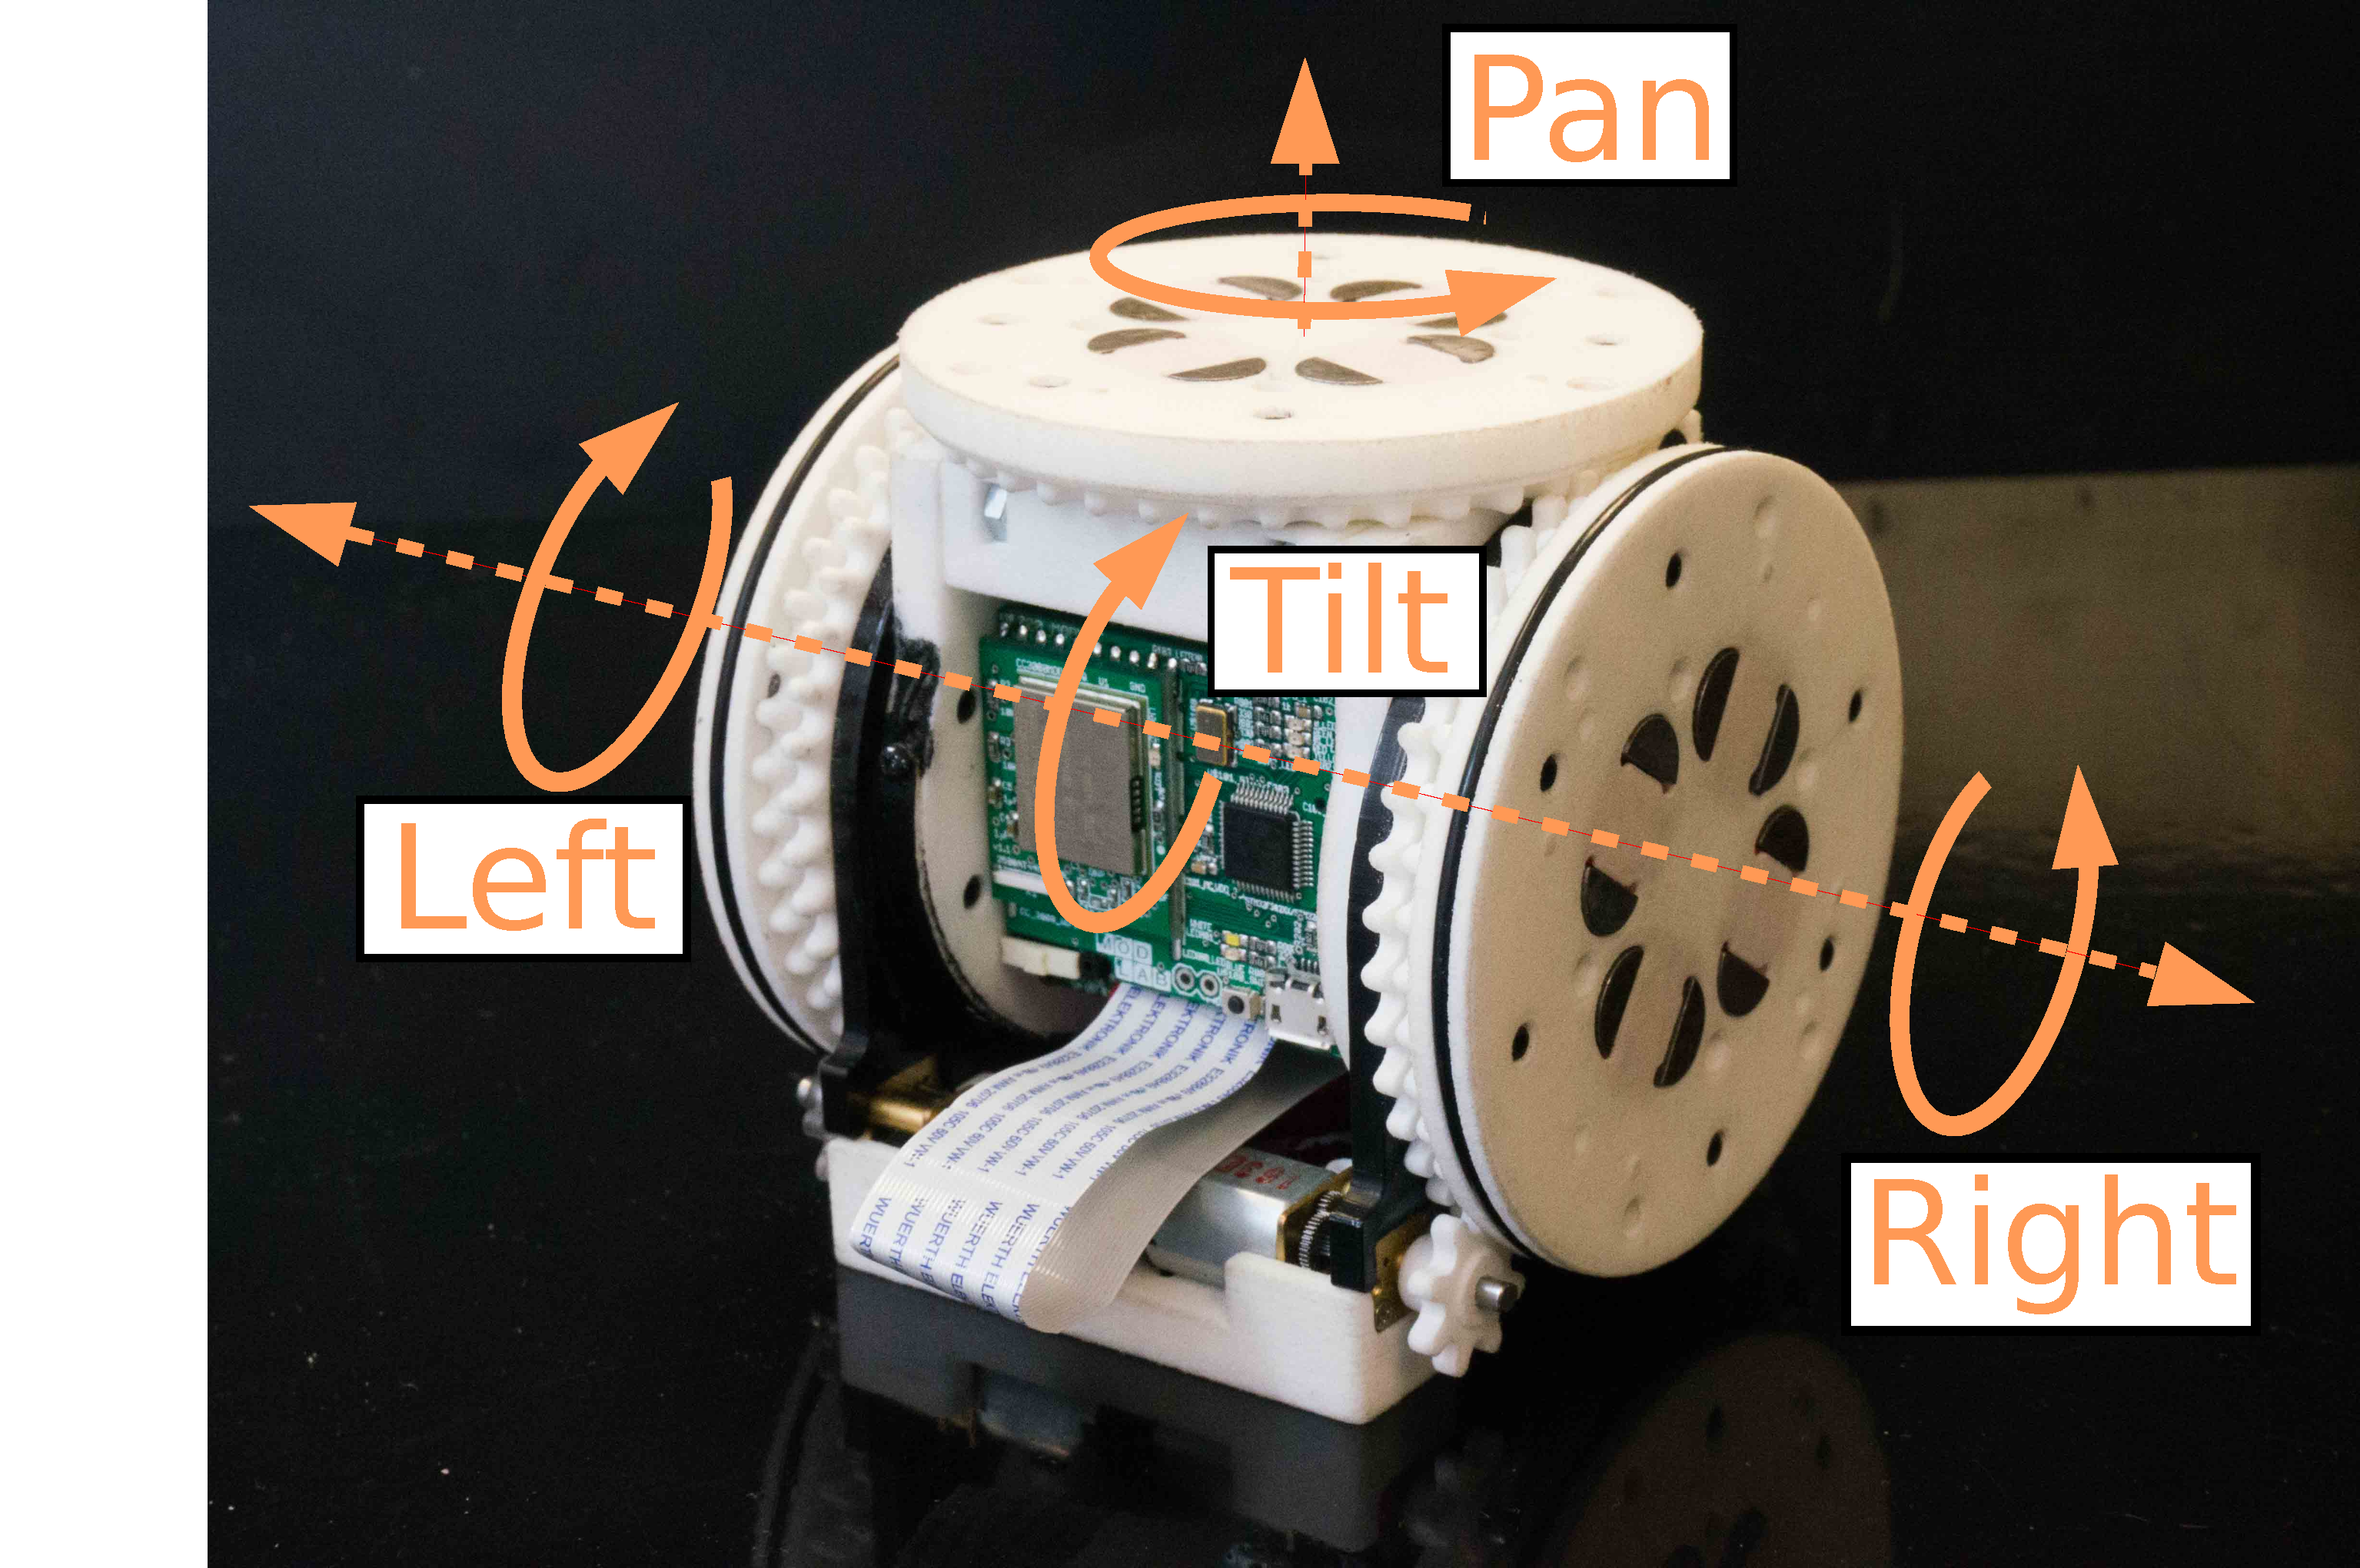
\includegraphics[height=1.5in]{images/smores_dof.pdf}
\end{center}
\caption{SMORES-EP module}
\label{fig:smores-module}
\end{figure}
%

\subsection{Brain Module} % (fold)
\label{sec:sensor_module}
%
SMORES-EP modules have very limited onboard computation, and no sensors that allow them to gather information about their environment.  To allow the robot to operate autonomously in unknown environments, we extend the SMORES-EP hardware system by introducing a brain module equipped with sensors and a computer, shown in Figure~\ref{fig:sensor-module}.

The body of the brain module is a $160\times80\times80mm$ box, roughly the size of two SMORES-EP side-by-side.  The brain module can be configured to provide attachment points on the back, front, or bottom that allow easy connection to SMORES-EP modules or passive cubes.

Computation is provided by an UP computing board with an Intel Atom 1.92 GHz processor, 4 GB memory, and a 64 GB hard drive. A USB WiFi adapter provides network connectivity. A front-facing XTION-Pro Live camera mounted on top of the brain module body provides RGB-D data, enabling the robot to explore and map its environment and recognize objects of interest.  A thin stem extends $30cm$ above the top of the body, supporting a downward-facing Microsoft Lifecam webcam mounted at $40^\circ$ to vertical.  This camera provides a view of a  $1m\times0.75m$ area in front of the brain module, and is used to track AprilTag fiducials during reconfiguration. A $7.4v$, $3600mAh$ LiPo battery provides about 1.5 hours of up time.
%
% Sensor Module Figure
\begin{figure}
\begin{center}
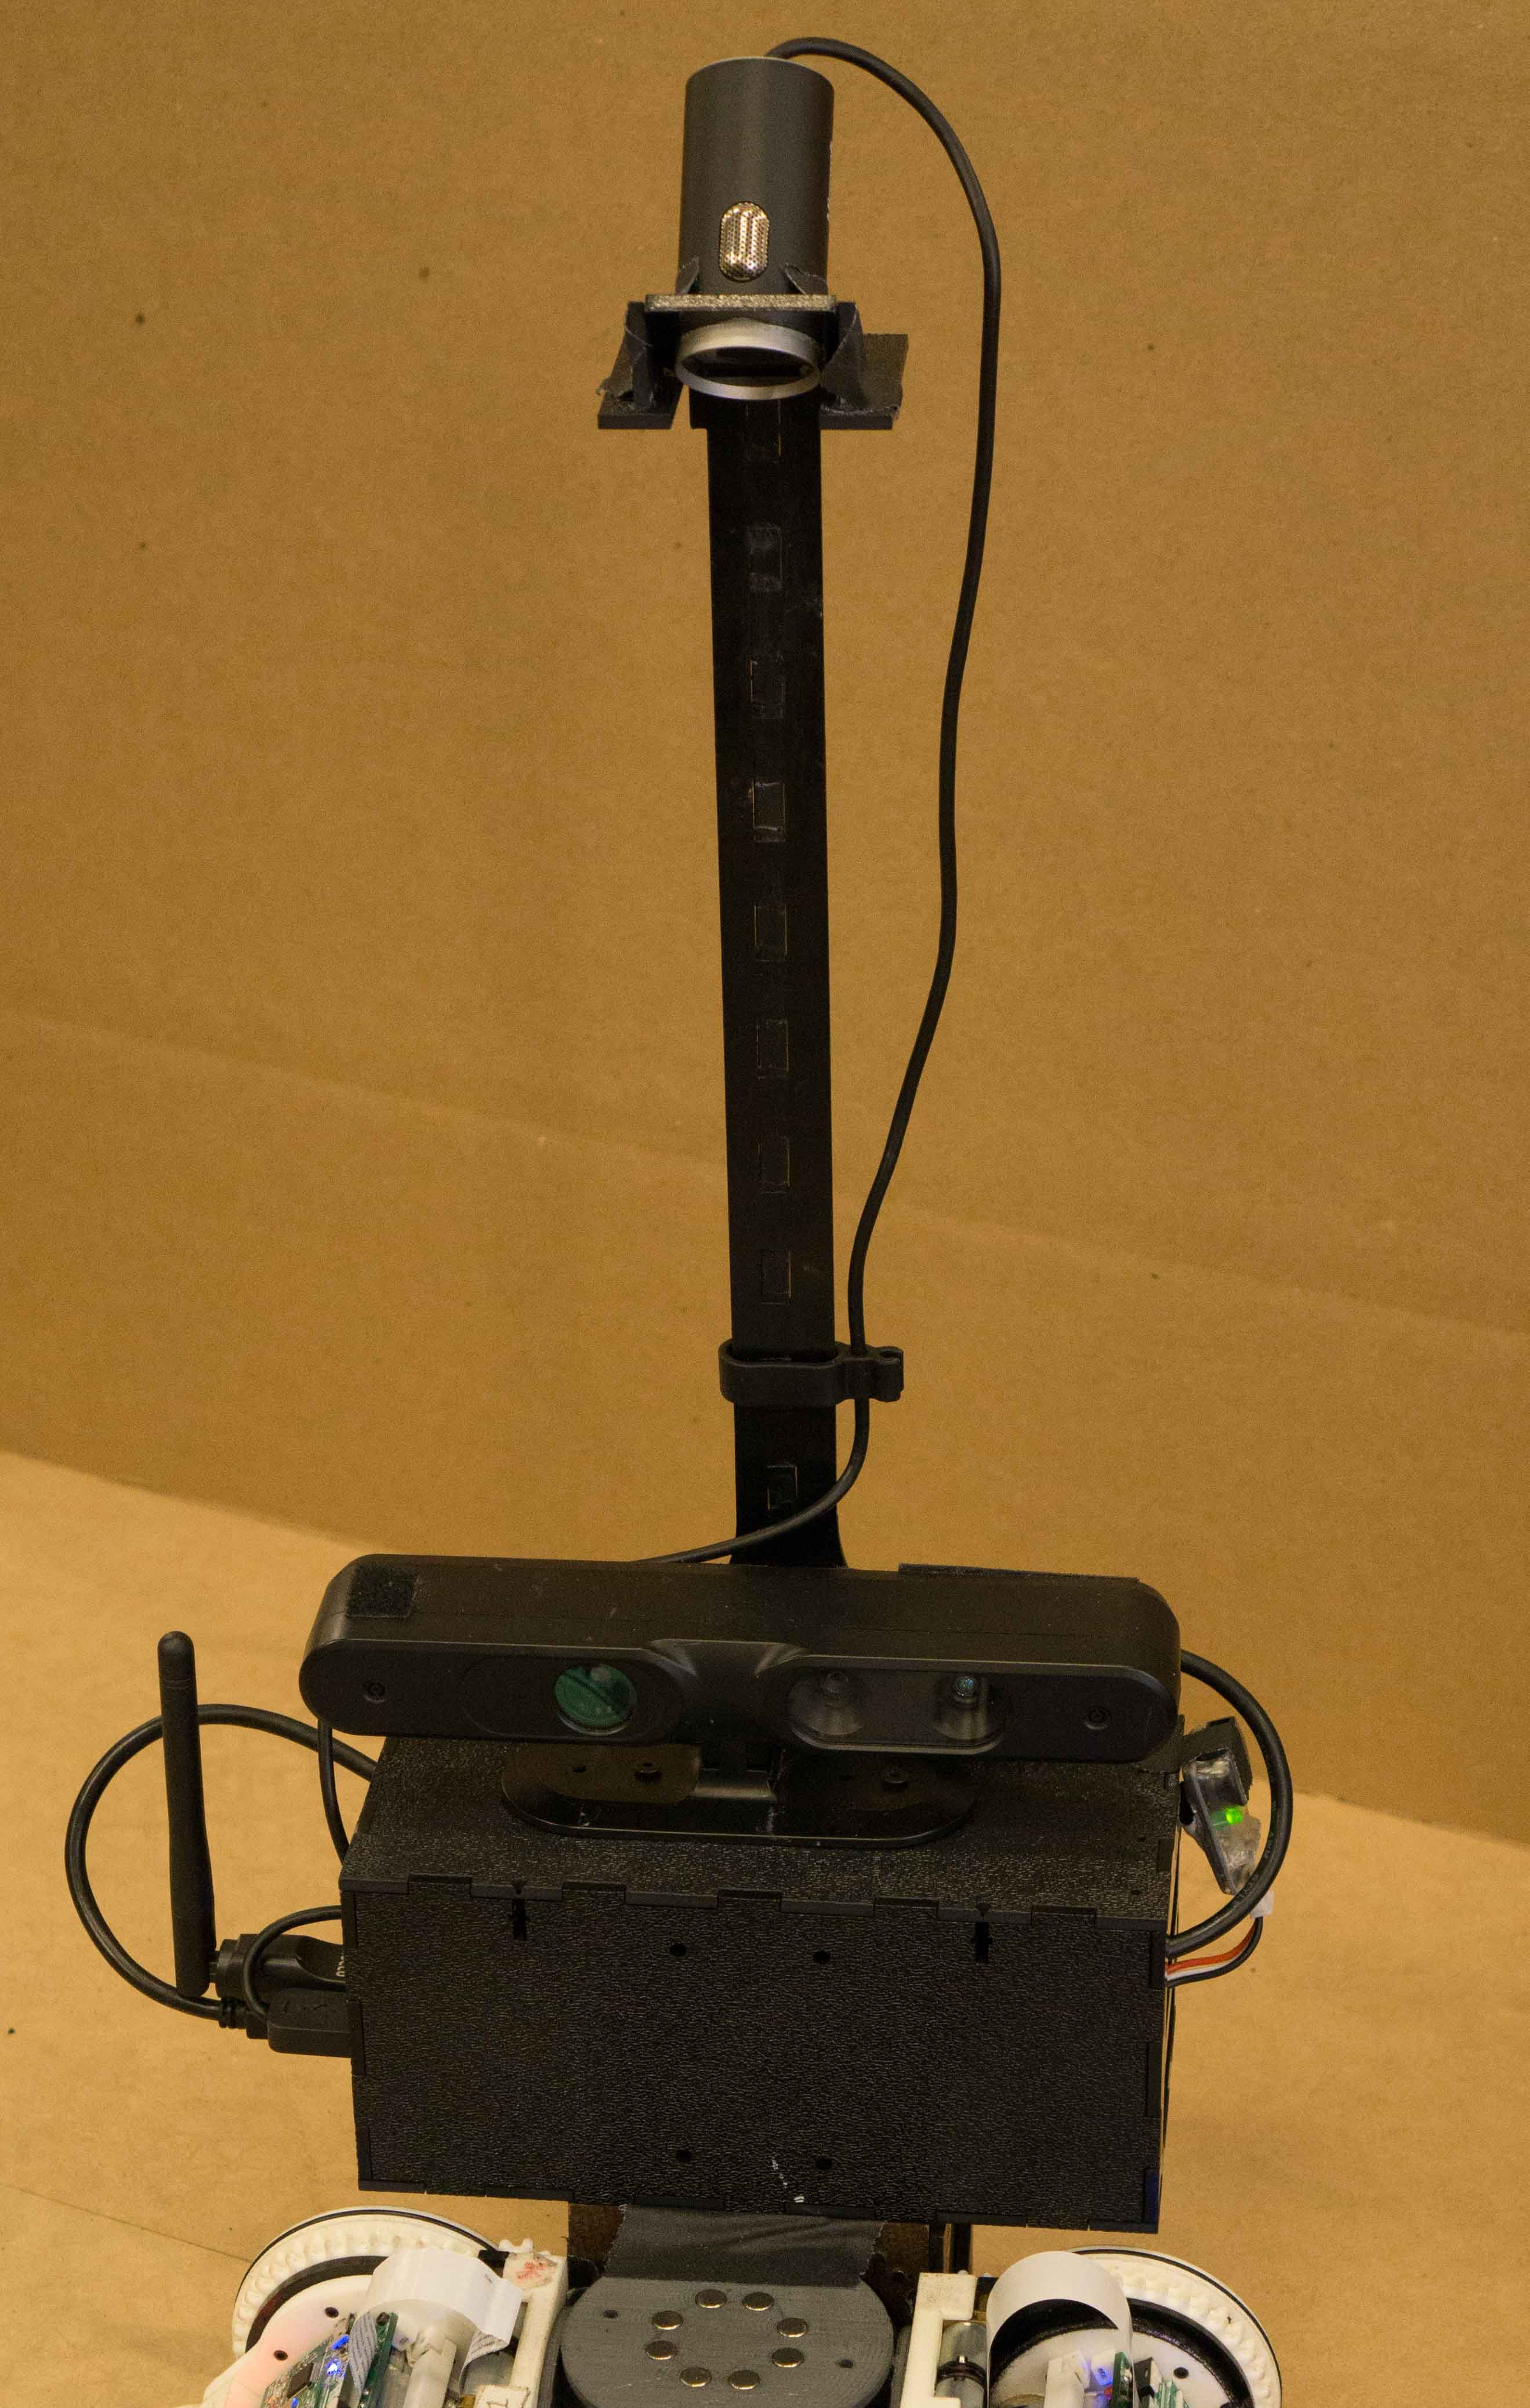
\includegraphics[width=0.3\textwidth]{images/sensor_module.jpg}
\caption{Brain Module}
\label{fig:sensor-module}
\end{center}
\end{figure}


%     ____                            __  _
%    / __ \___  _____________  ____  / /_(_)___  ____
%   / /_/ / _ \/ ___/ ___/ _ \/ __ \/ __/ / __ \/ __ \
%  / ____/  __/ /  / /__/  __/ /_/ / /_/ / /_/ / / / /
% /_/    \___/_/   \___/\___/ .___/\__/_/\____/_/ /_/
%                          /_/
\section{Mapping and Exploration}
\label{sec:exploration}
%
%Our system provides a robust suite of perception algorithms to inform control and decision-making in unknown environments.  This suite of tools serves three major functions.  First, it enables exploration, allowing the robot to map its environment, localize, and avoid obstacles.  Second, it provides the capability to recognize objects and regions of interest related to the desired task.  Third, it provides functions that characterize environment properties, providing information that allows appropriate configurations and behaviors to be selected from the design library.

%Since the proposed system performs tasks in unknown environments and conditions, a robust suite of perception algorithms is required to inform control and decision-making. The robot must have the ability to explore and build a map of its environment while avoiding obstacles and tracking its pose. The system must be able to recognize objects and regions of interest related to the desired task. Finally, the system must characterize the environment in terms of configuration capabilities. Features in the environment may restrict which robot configurations can viably perform parts of the high-level task, such as retrieving an object or navigating to a waypoint. The system needs to recognize these features to be able to intelligently choose the appropriate robot configuration for performing the task.

Exploration of unknown environments is a core functionality of our system.  While the methods used are not novel in the broader context of robotics,  this system represents one of the first modular robot systems capable of exploring and operating in totally unknown environments.

To facilitate the use of open source software and enable networking between components, the proposed system is built in a ROS framework\footnote{http://www.ros.org}. Mapping and robot pose are provided by a RGB-D SLAM software package called RTAB-MAP\cite{rtabmap}. A 3D map of the environment is incrementally built and stored in an efficient octree-based volumetric map using Octomap\cite{octomap}.

The system intelligently explores an unknown environment using using a new next best view planner for object exploration created by two of the authors\footnote{This work has been newly accepted for journal publication in 2017}. This planner directs the robot to explore its environment in a way that maximizes information gain while avoiding collision with obstacles. The algorithm uses the current volumetric map of the environment and estimates the next reachable sensor viewpoint that will observe the largest volume of undiscovered portions of objects. It also estimates the amount of information (in an entropy-reduction sense) that will be gained from a sensor measurement taken at that viewpoint. To integrate into the proposed system, the exploration algorithm is offered as a service that can be queried by the high-level planner when desired. A volumetric map of the environment and the reachable space of sensor viewpoints in that map must be provided to the algorithm. The algorithm then computes and returns the next best view for the sensor, which the high-level planner can then set as a navigation waypoint.

Note that the reachable space is dependent on the locomotion capabilities of the specific robot configuration. This information is associated with the configuration in the design library.

To identify objects of interest to a high-level task, our system provides tools to recognize color blobs and track their location in 3D.  Colors are recognized using CMVision\footnote{CMVision: http://www.cs.cmu.edu/$\sim$jbruce/cmvision/}, and tracked in 3D using depth information from the Xtion sensor\footnote{Lucas Coelho Figueiredo: https://github.com/lucascoelho91/ballFollower}.  This information is used to evaluate environment propositions in the high-level task, discussed in Section~\ref{sec:high-level}.  While we currently only provide object recognition by color, more sophisticated methods could easily be included. 
%

%    ______            _____          _____                 _ _____
%   / ____/___  ____  / __(_)___ _   / ___/____  ___  _____(_) __(_)_________
%  / /   / __ \/ __ \/ /_/ / __ `/   \__ \/ __ \/ _ \/ ___/ / /_/ / ___/ ___/
% / /___/ /_/ / / / / __/ / /_/ /   ___/ / /_/ /  __/ /__/ / __/ / /__(__  )
% \____/\____/_/ /_/_/ /_/\__, /   /____/ .___/\___/\___/_/_/ /_/\___/____/
%                        /____/        /_/
\section{Library of Configurations and Behaviors}
\label{sec:configuration-specifics}
%
SMORES-EP has the capability to \emph{self-reconfigure}: changing the connected structure of a cluster of modules to assume different shapes and capabilities.  In order to specify tasks for SMORES-EP (or any other self-reconfigurable robot) at a high level, we must abstract the robot in a way that captures the fact that its capabilities are a function of its configuration (connected structure). For the purposes of this work, we rely on a framework first presented in \cite{Jing2016}, which we summarize here.

In this framework, the entire modular robot system is treated as a single robot with capabilities defined by a design library. A library entry is defined as $l = (C,B_C,P_e,P_b)$ where:
\begin{itemize}
\item $C$ is the robot \emph{configuration}, specified by the connected structure of the modules.
\item $B$ is a \emph{behavior} that $C$ can perform. A behavior is a controller that commands the robot to perform a specific useful action. 
\item $P_b$ is a set of \emph{behavior properties} that describes what $B$ does. 
\item $P_e$ is a set of \emph{environment properties} that describe the environment in which this library entry is suitable. 
\end{itemize} 
%
In this work, we create five library entries for two different configurations,
listed in Table~\ref{table:1}. 
The ``Tank'' configuration shown in Fig.~\ref{fig:dropoff} is capable of picking
up and dropping objects in ``free'' environment while driving on a flat plain as a
differential drive robot.
The ``Proboscis'' configuration shown in Fig.~\ref{fig:pink_grab} has
a long arm in front, and is suitable for reaching between obstacles in a narrow ``tunnel'' environment to grasp objects.
However, the locomotion ability of this configuration is limited to forward/backward
motion, making it unsuitable for general navigation.

This library-based framework allows us to specify tasks for modular robots at a high level. Environment
properties $P_e$ specify when a given behavior can be used, and are a function of
the sensed environment.  In Section~\ref{sec:environment-characterization}, we discuss
the methods we use to extract environment properties from 3D sensor data. When we
specify tasks at the high level, we use behavior properties $P_b$ to describe an
action we want the robot to take without explicitly specifying which configuration
or behavior to use.

For example, if a task specification requires the robot to execute a $pickUp$ behavior, our system could select  either the Tank or Proboscis configurations to perform the action, since both have behaviors with $P_b=pickUp$. To make the decision, the system will consider the current environment properties, $P_e$, extracted from sensor data.  In the case that $P_e=tunnel$, only the Proboscis configuration can be used, and the robot will take  reconfigure to form the Proboscis if it is not already in that configuration.

Since self-reconfiguration is time-consuming, decisions are biased toward behaviors associated with the current configuration whenever possible, so that the robot only reconfigures when it is necessary to complete a task.
%
\begin{table}
\centering
\begin{tabular}{ |c|c|c| } 
 \hline
 \multirow{2}{6em}{Configuration} & Behavior & Environment \\
 & properties & properties \\
 \hline
 Tank & Pick up & Object in ``free'' environment \\\hline
 Tank & Drop & Drop-off zone in ``free'' environment \\\hline
 Tank & Drive & Flat plain\\ \hline
 Proboscis & Pick up & Object in ``tunnel'' or ``free'' environment \\ \hline
 \multirow{2}{4em}{Proboscis} & \multirow{2}{2em}{Drop} & Drop-off zone in \\
 & & ``tunnel'' or ``free'' environment \\ 
 \hline
\end{tabular}
\caption{A library of robot behaviors}
\label{table:1}
\end{table}

%
% subsection sensor_module (end)
% section hardware (end)
%

\section{Environment Characterization}
\label{sec:environment-characterization}
%
As discussed in Section~\ref{sec:configuration-specifics}, the system takes environment features into account when selecting an appropriate library entry to complete an action. Our perception suite includes functions that process the 3D information to identify environment properties.

%In order to intelligently choose appropriate configurations when performing tasks, the robot must perceive and characterize its environment into a discrete set of environment types that correspond with configuration capabilities. The proposed system includes a perception component that discretely characterizes the environment for the purpose of retrieving an object. This characterization can then be used by the high-level planner to determine the appropriate configuration and gait for successful object retrieval. 

Currently, the perception suite includes functions to recognize three types of environments relevant to object retrieval tasks, shown in Figure \ref{fig:characters}.  When an object is recognized in the environment, the 3D information about its surroundings is evaluated. If the object's position is higher than a threshold height, the environment is characterized as the ``ledge,'' likely requiring a library entry that can reach up to the top of the ledge to retrieve the object.
If the object is on the ground, an occupancy grid is created around it, and all grid cells within a robot-radius of obstacles are denoted unreachable (as shown in Figure~\ref{fig:characterization}). The closest reachable point to the object within $20^o$ of the robot's line of sight to the object is selected. If the distance from this point to the object is greater than a threshold value, the environment is characterized as a ``tunnel,'' likely requiring a configuration that is narrow enough to move between the surrounding obstacles to retrieve the object.
If the environment surrounding the object does not meet the criteria for either a ``ledge'' or ``tunnel,'' it is characterized as ``free.''
%If the environment type is ``tunnel'', the algorithm also selects a navigation waypoint at which the robot can reconfigure before retrieving the object. This waypoint is calculated by extending the closest point farther away from the object to be retrieved (red arrow in Figure \ref{fig:characterization}). This information is passed to the high-level planner for use in controller synthesis.
%
% Environment types figure
\begin{figure}[t]
      \centering
      \begin{subfigure}[t]{0.15\textwidth}
        \includegraphics[width=\textwidth]{images/free.png}
        %\label{fig:obja}
        \caption{\textbf{``free'}' environment}
    \end{subfigure}
    \begin{subfigure}[t]{0.15\textwidth}
        \includegraphics[width=\textwidth]{images/ledge.png}
        %\label{fig:objb}
        \caption{\textbf{``ledge''} environment}
    \end{subfigure}
        \begin{subfigure}[t]{0.15\textwidth}
        \includegraphics[width=\textwidth]{images/tunnel.png}
        %\label{fig:objb}
        \caption{\textbf{``tunnel''} environment}
    \end{subfigure}
      \caption{Environment characterization types for object retrieval.}
      \label{fig:characters}
   \end{figure}
%
% Characterization method figure
\begin{figure}
\begin{center}
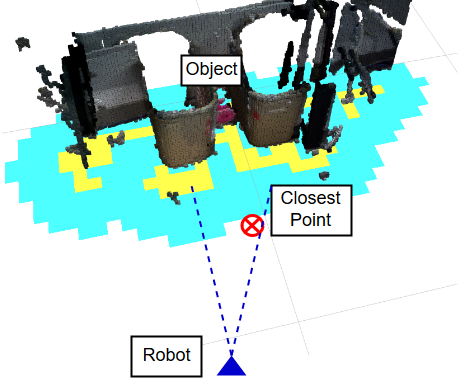
\includegraphics[width=0.4\textwidth]{images/characterization.png}
\caption{\textbf{Tunnel} environment characterization method.}
\label{fig:characterization}
\end{center}
\end{figure}

%     ____                        _____                        __  _
%    / __ \___  _________  ____  / __(_)___ ___  ___________ _/ /_(_)___  ____
%   / /_/ / _ \/ ___/ __ \/ __ \/ /_/ / __ `/ / / / ___/ __ `/ __/ / __ \/ __ \
%  / _, _/  __/ /__/ /_/ / / / / __/ / /_/ / /_/ / /  / /_/ / /_/ / /_/ / / / /
% /_/ |_|\___/\___/\____/_/ /_/_/ /_/\__, /\__,_/_/   \__,_/\__/_/\____/_/ /_/
%                                   /____/
\section{Reconfiguration}
\label{sec:reconfiguration}
%
Reconfiguration refers to the process of changing the connective topology of an MSRR system's modules in order to change its morphology.  SMORES-EP is capable of all three classes of modular self-reconfiguration (chain, lattice, and mobile reconfiguration) \cite{Davey2012,yim2003modular}.  For the purposes of this work, we have developed tools for mobile reconfiguration with SMORES-EP, taking advantage of the modules' ability to drive on flat surfaces as described in section \ref{sec:hardware}.

Determining the relative position of modules during mobile self-reconfiguration is an important challenge. As discussed in Section~\ref{sec:related-work}, past systems have relied on offboard global positioning systems \cite{Paulos2015} or distributed approaches, in which sensors are mounted on each disconnected set of modules \cite{Yim2007}.  Our localization method is centralized, using an RGB camera carried by the robot to track AprilTag fiducials mounted to individual modules.  As discussed in Section~\ref{sec:hardware}, the camera provides a view of a $1m\times0.75m$ area on the ground in front of the brain module.  Within this area (which we call the \emph{reconfiguration zone}), any module equipped with an AprilTag marker can detach from the cluster, drive to another location, and reattach to the cluster, provided that both of its wheels were in contact with the ground in its starting position.% \TODO{Get accurate number for height and FoV.}

\subsection{Reconfiguration Procedure}
Given an initial configuration and a goal configuration, our reconfiguration controller commands a set of modules to disconnect, move and reconnect in order to form the new topology of the goal configuration. The process consists of three stages: i) Pre-reconfiguration, ii) Module Movement, iii) Post-reconfiguration.

\paragraph{Pre-reconfiguration} In the pre-reconfiguration stage, the robot takes actions to establish the conditions needed for reconfiguration.  It begins by confirming that the reconfiguration zone is a flat surface free of obstacles (other than the modules themselves).  If the robot is carrying an object, it drops the object outside of the reconfiguration zone. It then  sets its joint angles so that all modules that need to detach have both of their wheels on the ground, ready to drive. Once these conditions are established, module movement begins.

\paragraph{Module Movement} During this stage, the topology of the cluster changes as a sequence of module movement operations are performed.  Each operation changes the topology of the cluster by detaching a module from the cluster, driving, and re-attaching at its new location in the goal configuration, as shown in Figure~\ref{fig:reconf}.

In order to transform from an initial configuration to a goal configuration, a feasible reconfiguration plan (sequence of module movement operations) must be supplied to the reconfiguration software before reconfiguration begins.  Each configuration in the library has an associated set of reconfiguration plans that allows it to transform to other configurations in the library.  Currently, reconfiguration plans are created by hand.  In the future, existing assembly planning algorithms (\cite{Werfel2007,Seo2013}) could be adapted to generate reconfiguration plans automatically.

% We denote a module movement operation as $MP=\left(m, m_d, m_a, f_m^d, f_m^a, f_{m_d}, f_{m_a}, \sigma \right)$ where:
% \begin{itemize}
% \item $m$ is the module whose location will be changed in this module operation.
% \item $m_d$ is the module that connects with $m$ before the operation.
% \item $m_a$ is the module that connects with $m$ after the operation. Notice $m_d$ and $m_a$ can be the same module. 
% \item The face $f_m^d$ of module $m$ connects with the face $f_{m_d}$ of module $m_d$ before the operation.
% \item The face $f_m^a$ of module $m$ connects with the face $f_{m_a}$ of module $m_a$ after the operation. Notice $f_m^d$ and $f_m^a$ can be the same face. In this work, we assume $f_m^a$ can only be the front or the back face of the module $m$.
% \item $\sigma$ is the path that module $m$ will follow during the operation.
% \end{itemize}

To travel from its initial location to its final location, a module uses its left and right wheels to move by differential-drive.  Because the reconfiguration zone is free of obstacles, collision-free paths can be pre-computed and stored as part of the reconfiguration plan.  Paths can also be computed at runtime if desired.  AprilTag localization allows the robot to follow the path.

Several techniques were developed to ensure reliable connection and disconnection during reconfiguration.  When a module disconnects from the cluster, the electro-permanent magnets on the connected faces are turned off.  To guarantee a clean break of the magnetic connection, the disconnecting module bends its tilt joint up and down, mechanically separating itself from the cluster. During docking, accurate alignment is crucial to the strength of the magnetic connection \cite{tosun2016design}.  For this reason, rather than driving directly to its final docking location, a module instead drives to a pre-docking waypoint directly in front of its docking location.  At the waypoint, the module spins in place slowly until its heading is perfectly aligned with the dock point, and then drives in straight to attach. To guarantee a good connection, the module intentionally overdrives its dock point, pushing itself into the cluster while firing its magnets.
%
\begin{figure}[t]
\begin{center}
  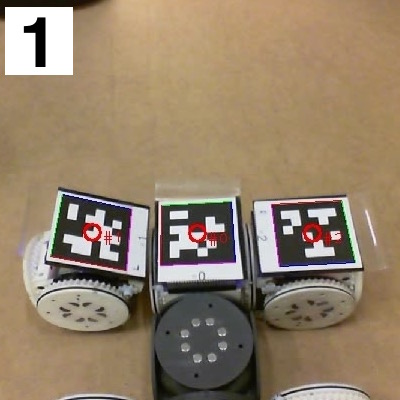
\includegraphics[width=0.32\columnwidth]{images/reconf_detach.jpg}
  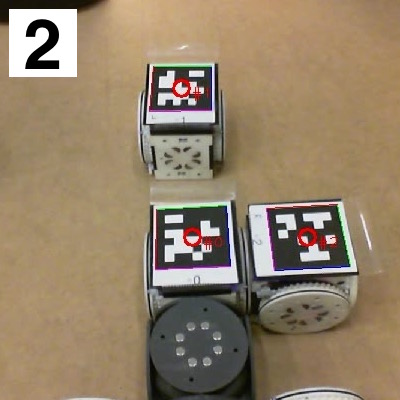
\includegraphics[width=0.32\columnwidth]{images/reconf_waypoint.jpg}
  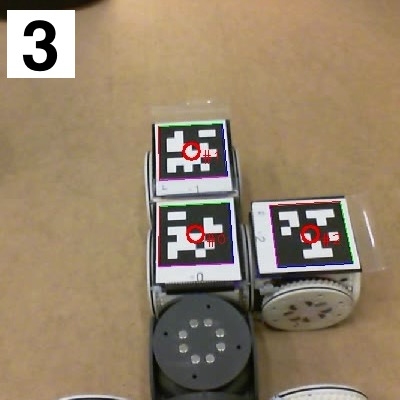
\includegraphics[width=0.32\columnwidth]{images/reconf_attach.jpg}
  \caption{Module movement during reconfiguration. (1) Left module detaches from cluster. (2) Module drives to waypoint, and spins to establish perfect heading. (2) Module drives straight in to dock point, and reattaches.}
  \label{fig:reconf}
\end{center}
\end{figure}

\paragraph{Post-reconfiguration} Once all module movement operations have completed and the goal topology is formed, the robot sets its joints to appropriate angles for the goal configuration to begin performing desired behaviors, and if necessary, the robot picks up any objects it dropped. This completes the reconfiguration process. 
%
%     __  ___       __          __                   __
%    / / / (_)___ _/ /_        / /   ___ _   _____  / /
%   / /_/ / / __ `/ __ \______/ /   / _ \ | / / _ \/ /
%  / __  / / /_/ / / / /_____/ /___/  __/ |/ /  __/ /
% /_/ /_/_/\__, /_/ /_/     /_____/\___/|___/\___/_/
%         /____/
%%
\section{High-Level Planner}
\label{sec:high-level}
%
% Automaton
%\begin{figure}
%\begin{center}
%\includegraphics[width=0.4\textwidth]{images/autSimple.png}
%\caption{Planner Automaton}
%\label{fig:automaton}
%\end{center}
%\end{figure}

To bring together the actuation, sensing, and reconfiguration capabilities of  the  robot as a complete system for accomplishing  tasks, we employ an existing framework LTLMoP to automatically generate robot controllers from user-specified high-level instructions using formal methods \cite{DBLP:conf/iros/FinucaneJK10,DBLP:journals/trob/Kress-GazitFP09}.
LTLMoP allows us to use each component of our system as a low-level atomic controller and specify a wide-range of reactive robotic tasks as a set of high-level instructions using these controllers.
In this section, we will mainly discuss how we model our system in order to use LTLMoP to automatically generate a high-level controller for our desired robot task.

\subsection{Controller Synthesis}
We first abstract the system and environment as a set of Boolean propositions.
For example, the system proposition ``pickUp'' is \lt if the robot is currently picking up an object (and \lf otherwise), and
the environment proposition ``object'' is \lt if the robot is currently sensing an object of interest (and \lf otherwise).

LTLMoP supports a high-level language called Structured English that allows the robot task to be specified in terms of these propositions.
For example, Specification~\ref{spec:experiment} shows the high-level instructions from the user that direct the robot to explore a room, search and move any object of interest to a drop-off zone.
In addition to ``pickUp'', this specification uses the system propositions ``explore'', ``drop'', ``carry'', ``driveToDropoff'' and ``driveToObject,'' each of which represents a different robot action.
Moreover, environment proposition ``arrived'' is \lt if the robot arrives at its target location, and ``dropoffzone'' is \lt if the robot is currently sensing a drop-off zone.

\begin{spec}[h!]
\caption{Search and move any object of interest to the drop-off zone}
\label{spec:experiment}
\vspace{-0.1cm}
\small\setlength{\jot}{0pt}
\begin{fleqn}[3pt]
\leqnomode
\begin{subequations}
\renewcommand{\theequation}{\arabic{equation}} 
\makeatletter
\renewcommand\tagform@[1]{\maketag@@@{\ignorespaces#1\unskip\@@italiccorr}}
\makeatother
\hskip-10cm
\begin{alignat}{2}
&\text{{\bf carry} is set on {\bf pickup} and reset on {\bf drop}}&& \notag \\
&\text{if you are not activating ({\bf carry} or {\bf pickup} or {\bf drop}}&& \notag \\
&\hspace{1cm}\text{or {\bf driveToObject} or {\bf driveToDropoff}) then do {\bf explore}}&& \notag \\
&\text{if you are activating {\bf carry} and you are not sensing {\bf dropoffZone}}&& \notag \\
&\hspace{1cm}\text{then do {\bf explore}}&& \notag \\
&\text{do {\bf driveToDropoff} if and only if you are activating {\bf carry} }&& \notag \\
&\hspace{1cm}\text{and you are sensing {\bf dropoffZone}}&& \notag \\
&\text{do {\bf driveToObject} if and only if you are not activating {\bf carry} }&& \notag \\
&\hspace{1cm}\text{and you are sensing {\bf object}}&& \notag \\
&\text{do {\bf drop} if and only if you were activating {\bf driveToDropoff } }&& \notag \\
&\hspace{1cm}\text{and you are sensing {\bf arrived}}&& \notag \\
&\text{do {\bf pickup } if and only if you were activating {\bf driveToObject} }&& \notag \\
&\hspace{1cm}\text{and you are sensing {\bf arrived}}&& \notag \\
&\text{infinitely often not {\bf carry}}&& \notag
\end{alignat}
\end{subequations}
\end{fleqn}
\vspace{-0.4cm}
\end{spec}

Given a specification,  LTLMoP will synthesize a robot controller that satisfies the given robot task (if one exists). The controller synthesized is in the form of a finite state automaton. Each state is labeled with the values of all system propositions. Each transition between two states is labeled with the value of all environment propositions.

\subsection{Controller Execution}
Since the synthesized high-level controller is a discrete finite state automaton, we need to implement it continuously in order to control the robot to satisfy the given task. 

Each environment proposition is mapped to a low-level sensing program that gathers and processes the information from sensor

s in order to characterize the environment state. For example, the propositions ``object'' is mapped to a sensing program offered by exploration component in Section~\ref{sec:exploration} that returns \lt or \lf based on whether the robot can detect a predefined pink or green object with its camera.

Similarly, each system proposition is mapped to behavior properties that specify how the action should be performed. As explained in Section~\ref{sec:configuration-specifics}, behavior and environment properties determine which library entry should be used to implement a given action.
For example, to implement the ``pickUp'' proposition in Specification~\ref{spec:experiment}, the system can execute any behavior that has the $Pick up$  behavior property, and which also satisfies the current environment properties.  If the current robot configuration cannot execute an appropriate behavior, the robot will reconfigure to a different configuration that can.   

%Each system proposition is mapped to a low-level control program that commands the robot to perform some behaviors. For example, the proposition ``pickUp'' is mapped to a program that will be executed when ``pickUp'' is \ltnsp. The program command the robot to perform a predefined behavior that will pick up a small magnetic object in front of the robot.
% In each iteration, first we determine the value of each environment propositions by calling each corresponding sensing program.
% We then can find the next state in the finite state automaton by taking the transition that matches with the current values of all environment propositions.
% At last, we execute the corresponding control program based on the value of each system proposition specified in the next state and continue to the next iteration.

Execution of the high-level controller begins at the predefined initial state in the finite state automaton. In each iteration, the values of all environment propositions and and environment properties are determined by calling the corresponding sensing program. Then, we determine the next state in the finite state machine by taking the transition that matches the current value of all environment propositions.
The system then maps the system proposition specified in the next state to its set of behavior properties, and selects a behavior from the design library which satisfies both the behavior properties and current environment properties. If the robot is not currently in a configuration capable of executing the selected behavior, the system commands the robot to reconfigure. Finally, the behavior is executed, and program execution continues on to the next iteration. 

%For example, in Fig.~\ref{fig:automaton} we start in the top state and execute the ``explore'' program.
%If  the robot senses a pink object, the value of ``pinkObject'' is \lt and therefore the next state is the bottom right state. We then stop the ``explore'' program and execute the ``driveToObject'' program.

%     ______                     _                      __
%    / ____/  ______  ___  _____(_)___ ___  ___  ____  / /______
%   / __/ | |/_/ __ \/ _ \/ ___/ / __ `__ \/ _ \/ __ \/ __/ ___/
%  / /____>  </ /_/ /  __/ /  / / / / / / /  __/ / / / /_(__  )
% /_____/_/|_/ .___/\___/_/  /_/_/ /_/ /_/\___/_/ /_/\__/____/
%           /_/
\section{Experiment Results}
\label{sec:experiments}
%

We validated and demonstrated our system's capabilities with a real-world experiment in which a robot composed of SMORES-EP modules completed a complex, high-level task in an unknown environment.  The high-level task consisted of three different types of sub-tasks: explore the environment, find and retrieve all objects in the office, and deliver each to a drop-off zone. Figure \ref{fig:map} shows the environment layout used in the experiment, designed to represent a cluttered office. Two objects to be retrieved were used: one was placed in the open (a ``free'' environment type), and another was positioned between two obstacles (a ``tunnel'' environment). Obstacles, environment types, and locations of the objects and drop-off zone were unknown to the robot \textit{a priori}.

Five SMORES-EP modules, one Brain Module, and three passive cubes composed the robot for performing the task. The robot grasped objects using modules' electro-permanent magnets to attach to steel plates on the objects.
During the experiment, the high-level planner used the library of two configurations and five behaviors described in Section \ref{sec:configuration-specifics}.

% Map
\begin{figure}
\begin{center}
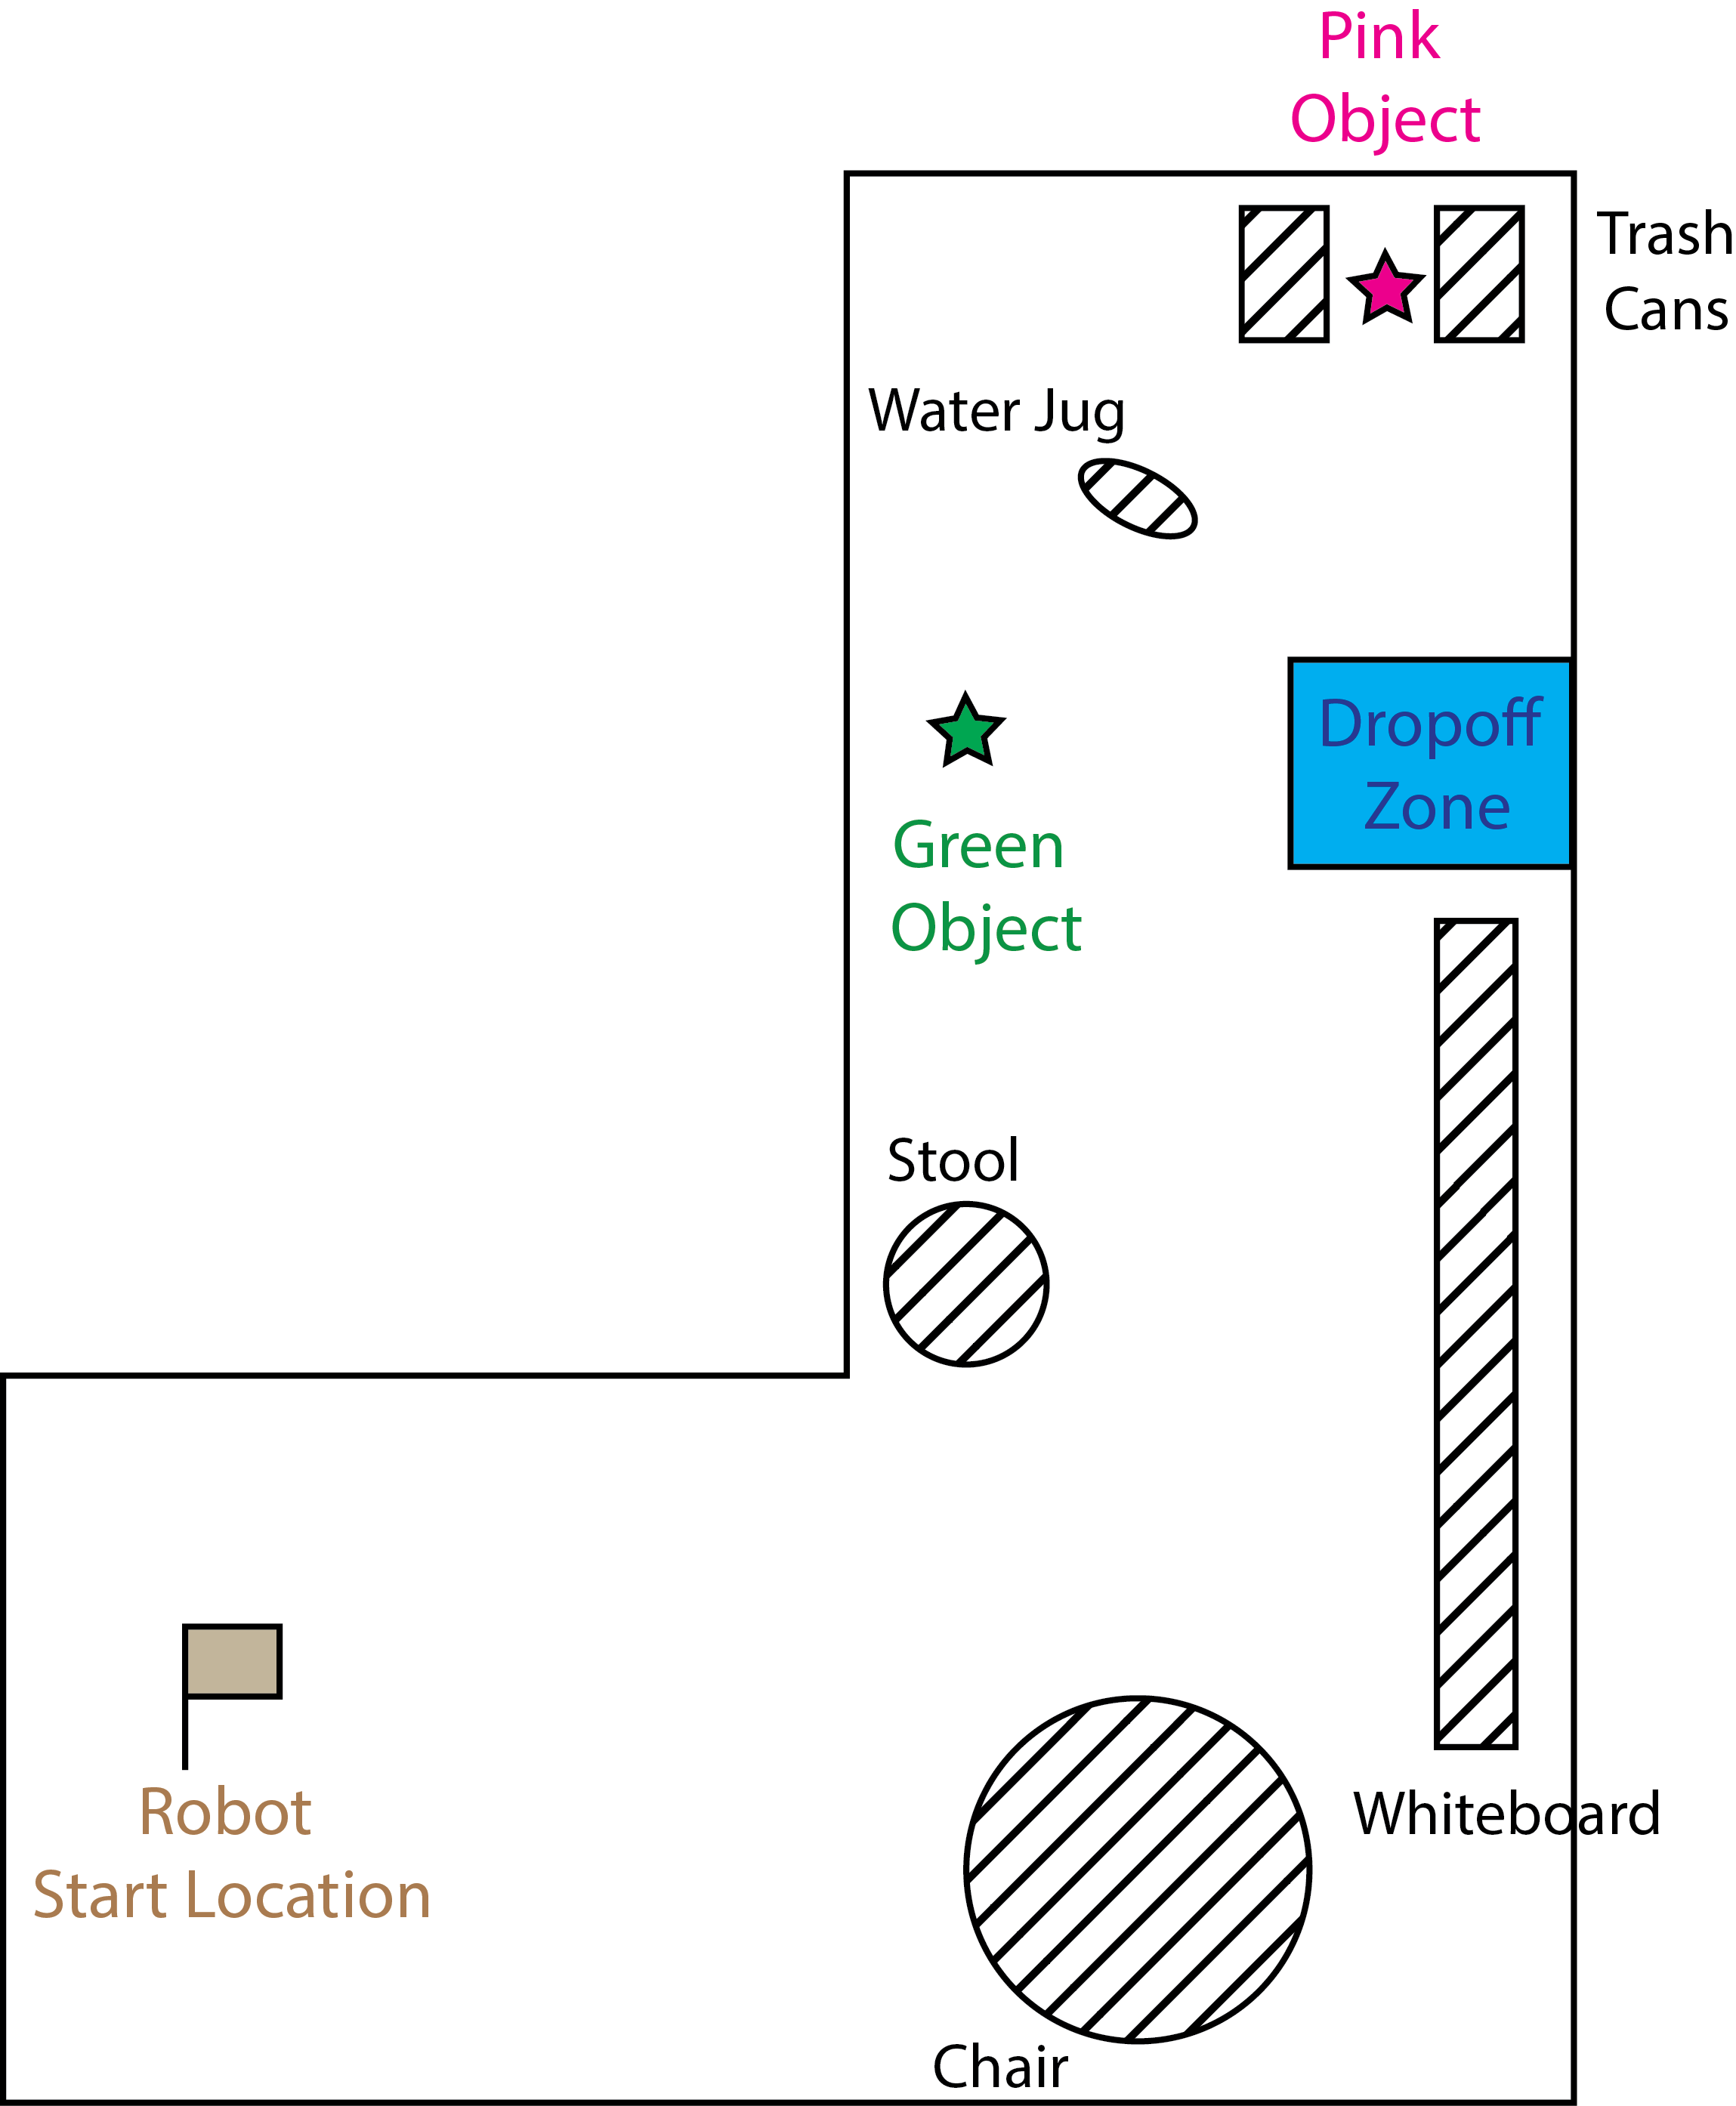
\includegraphics[width=0.4\textwidth]{images/RSSMap.png}
\caption{Diagram of experiment environment}
\label{fig:map}
\end{center}
\end{figure}

\begin{figure*}[t]
      \centering
      \begin{subfigure}[t]{0.32\textwidth}
        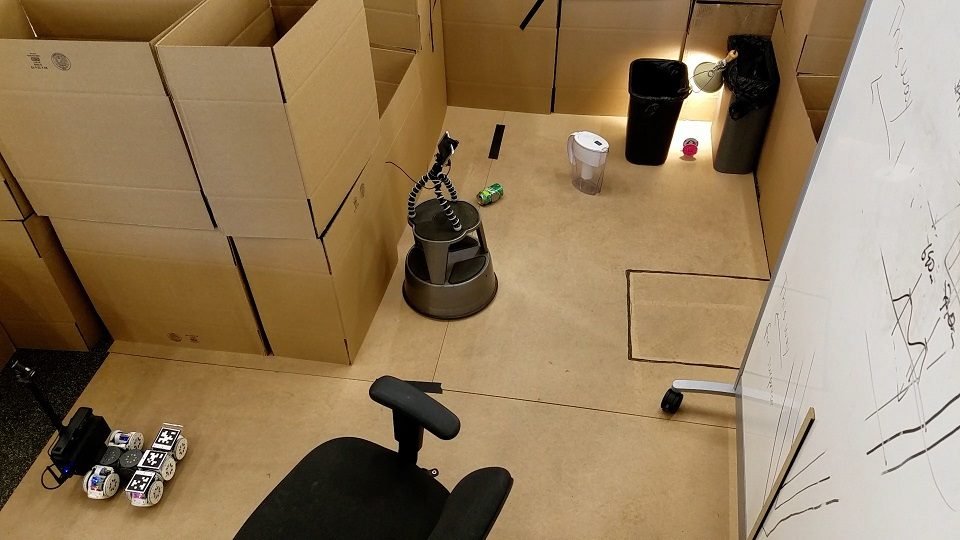
\includegraphics[width=\textwidth]{images/overhead_starting.jpg}
        %\label{fig:obja}
        \caption{Experiment setup and robot starting location}
    \end{subfigure}
    \begin{subfigure}[t]{0.32\textwidth}
        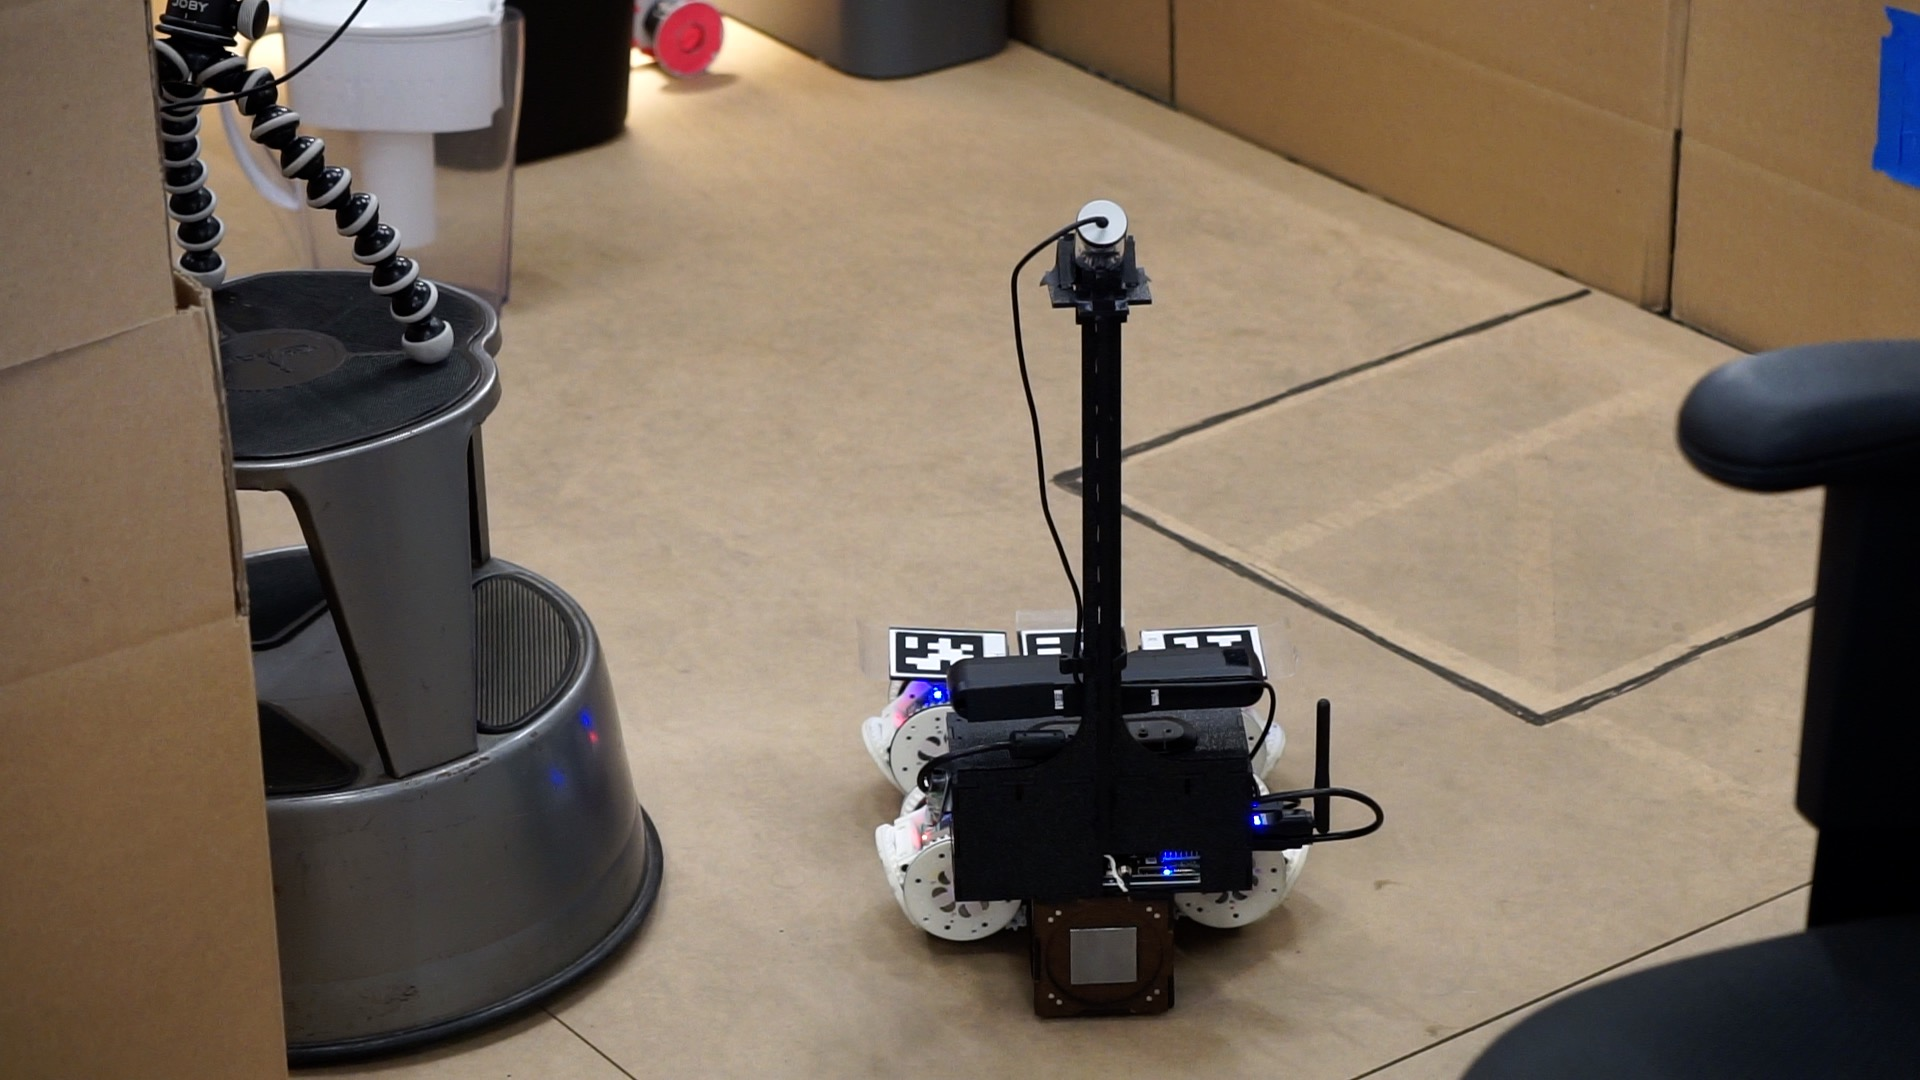
\includegraphics[width=\textwidth]{images/exploration.jpg}
        %\label{fig:objb}
        \caption{Exploring environment while searching for objects}
    \end{subfigure}
    \begin{subfigure}[t]{0.32\textwidth}
        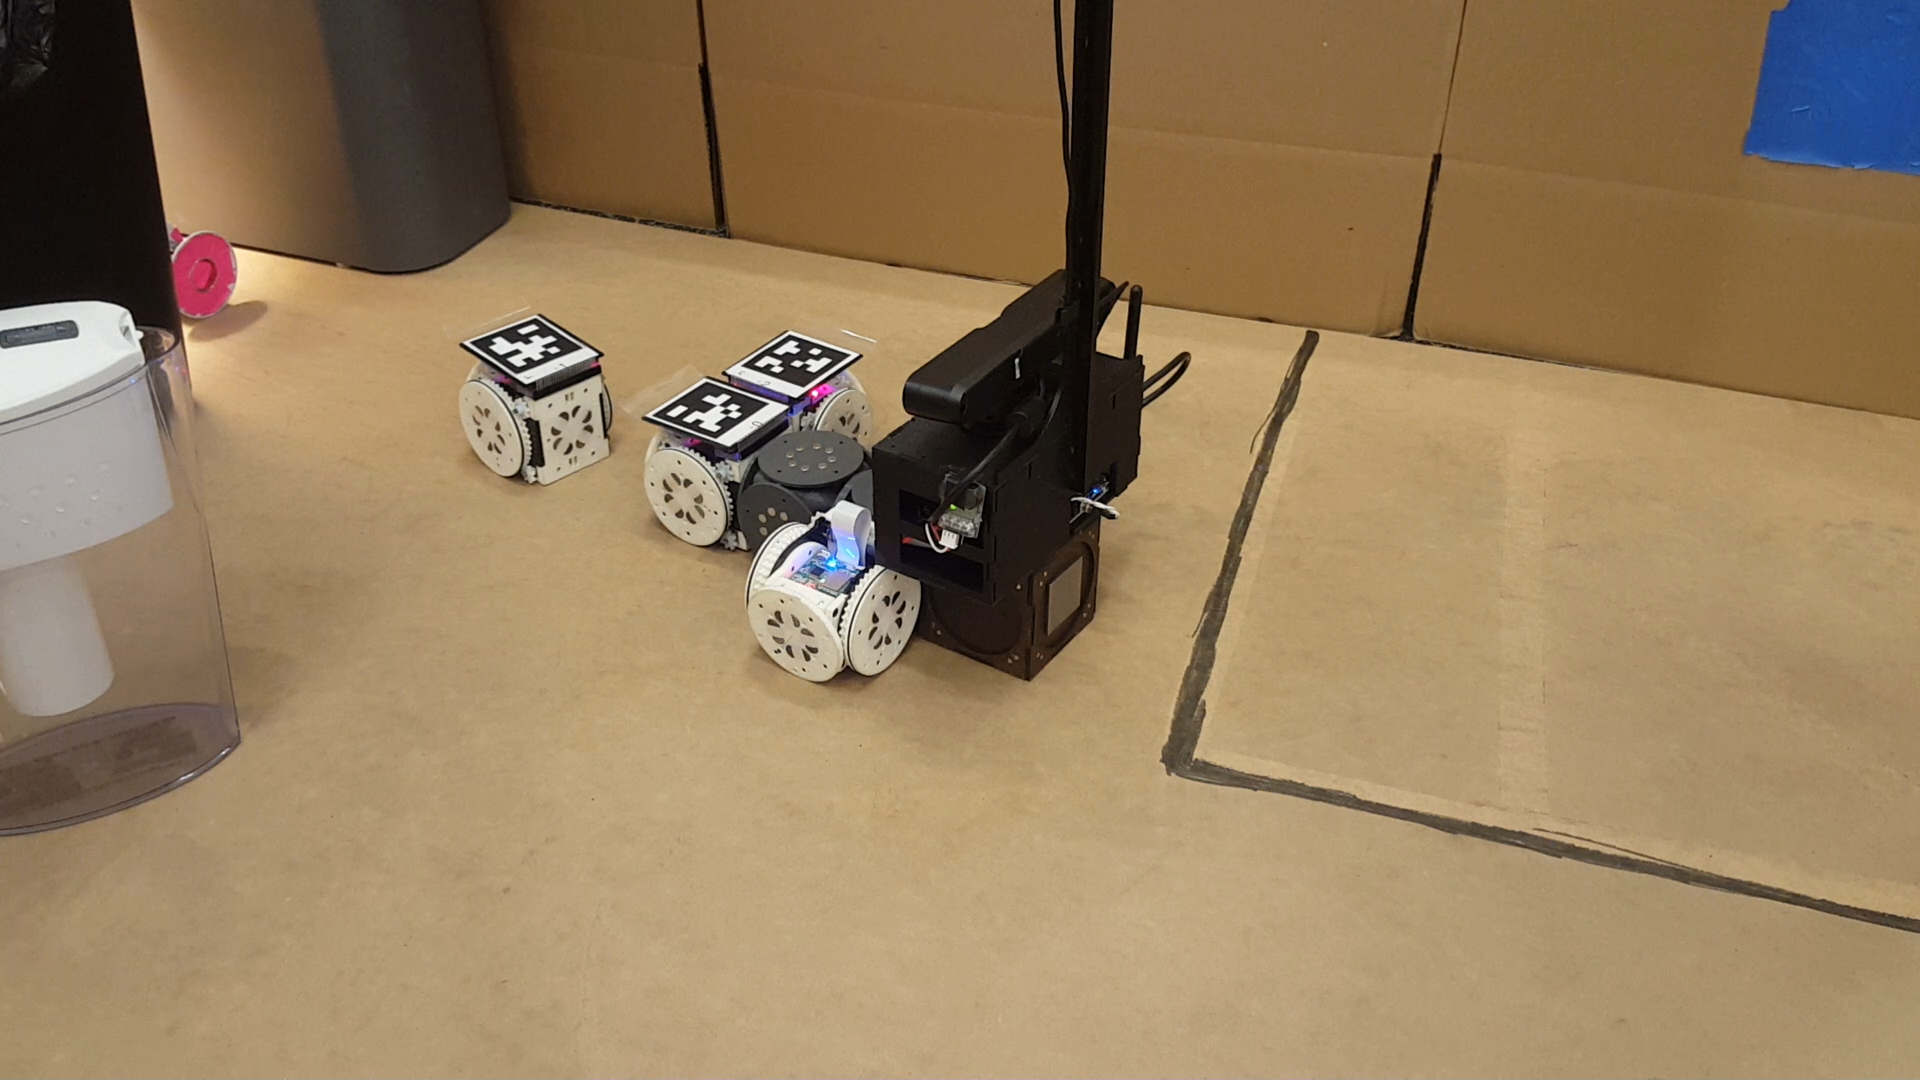
\includegraphics[width=\textwidth]{images/reconfiguration.png}
        %\label{fig:objb}
        \caption{Reconfiguring to retrieve pink object}
    \end{subfigure}
    \begin{subfigure}[t]{0.32\textwidth}
        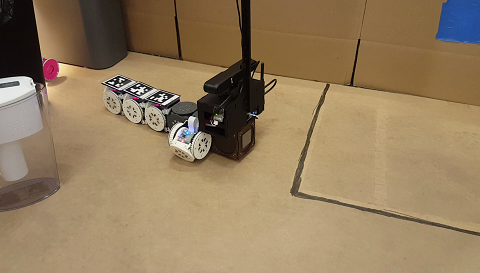
\includegraphics[width=\textwidth]{images/pink_retrieval.png}
        \caption{Retrieving pink object}
        \label{fig:pink_grab}
    \end{subfigure}
    \begin{subfigure}[t]{0.32\textwidth}
        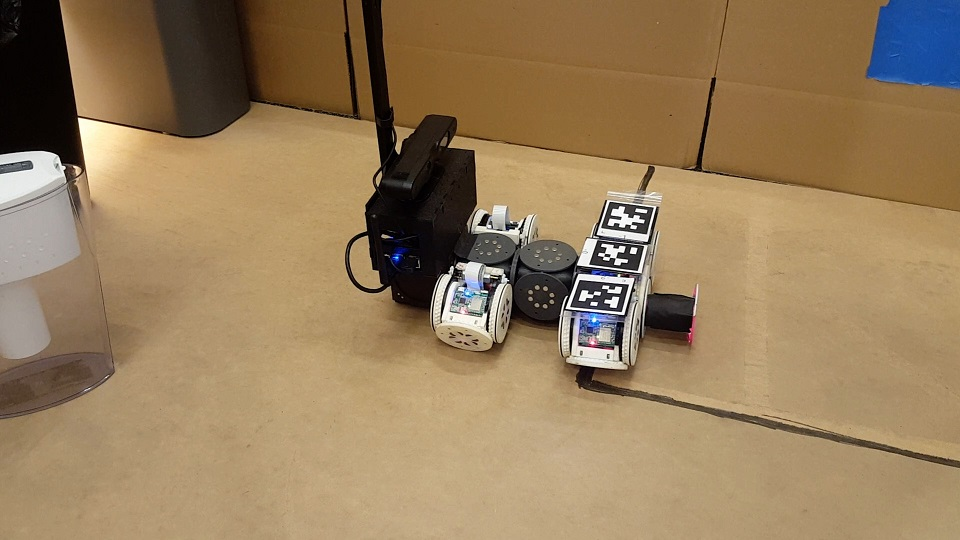
\includegraphics[width=\textwidth]{images/dropoff.jpg}
        \caption{Dropping off an object in the delivery zone}
        \label{fig:dropoff}
    \end{subfigure}
    \begin{subfigure}[t]{0.32\textwidth}
        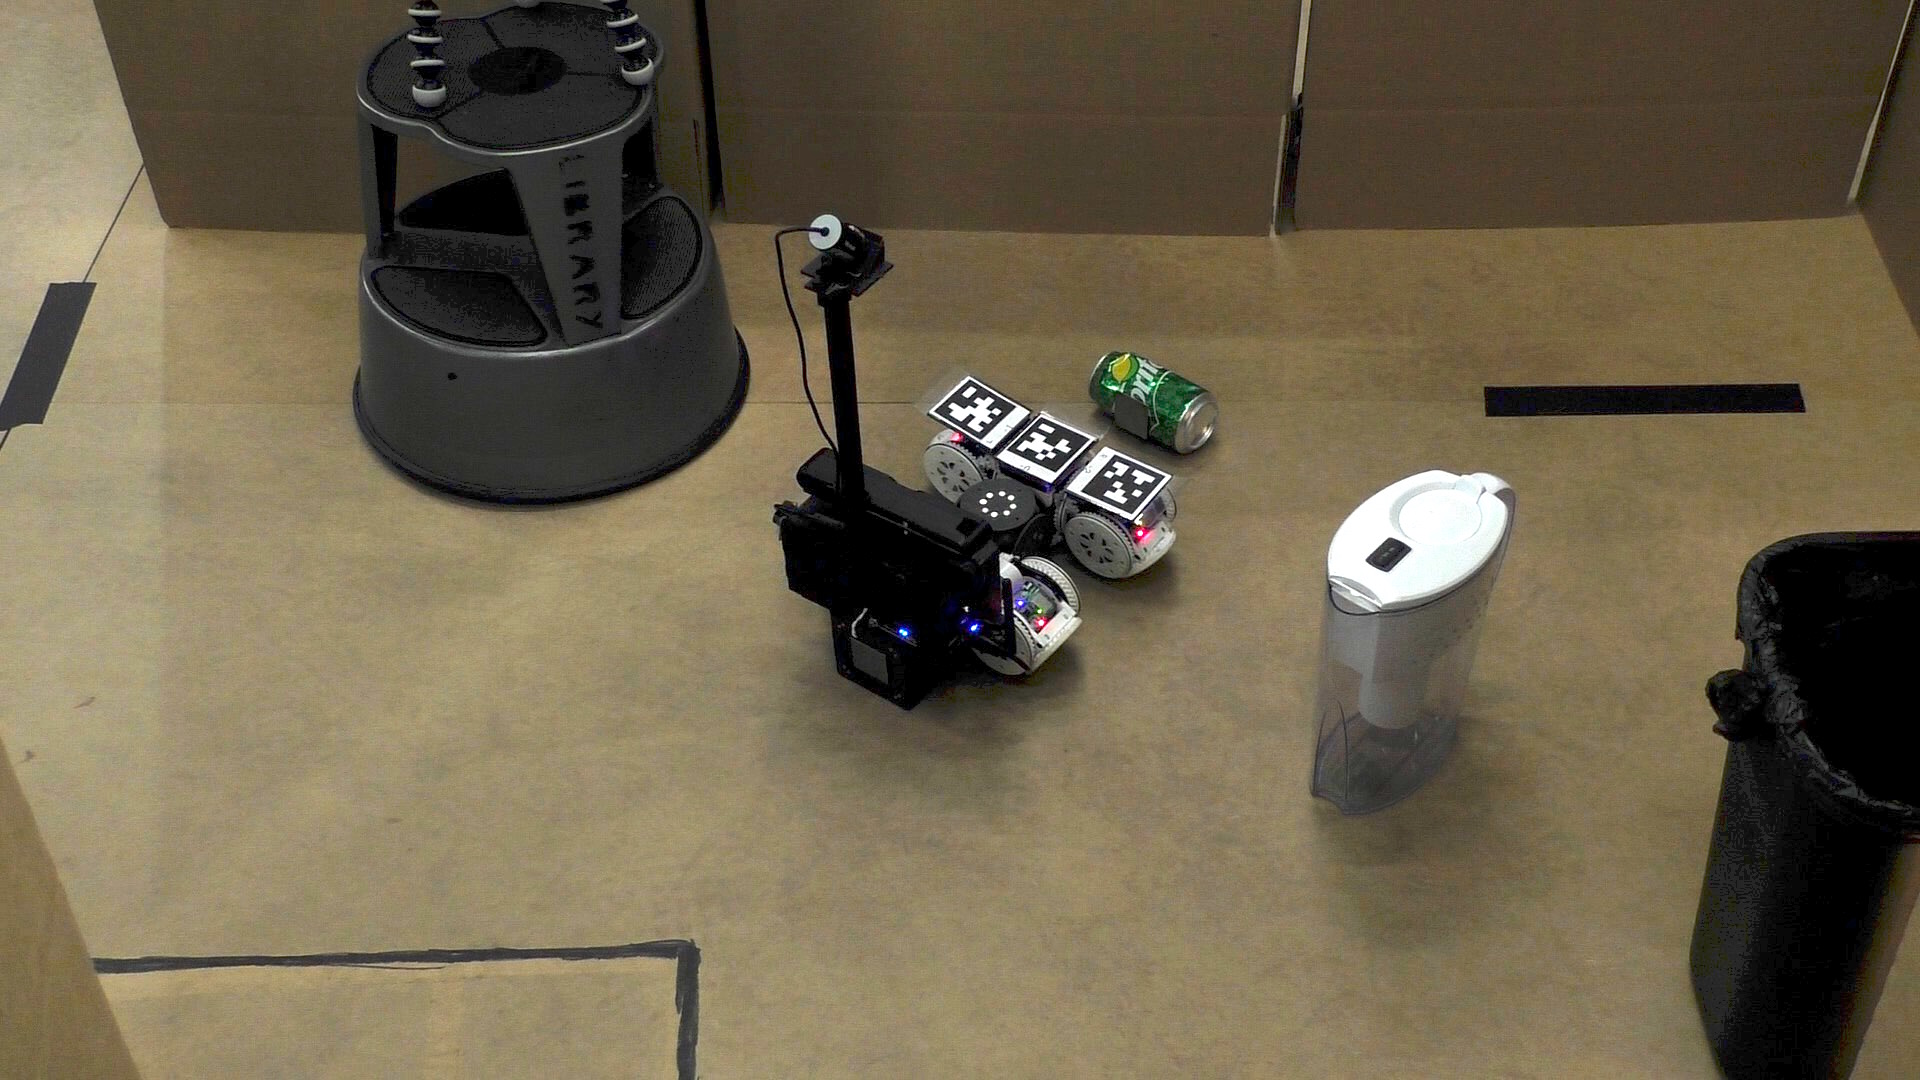
\includegraphics[width=\textwidth]{images/green_retrieval.jpg}
        %\label{fig:objb}
        \caption{Retrieving green object}
    \end{subfigure}
      \caption{Environment characterization types for object retrieval.}
      \label{fig:demo}
   \end{figure*}




Figure \ref{fig:demo} shows snapshots from the experiment run. A video of the entire experiment is available as an attachment to this paper. The starting location prevented the robot from seeing the objects initially, forcing it to explore the environment to search for them. After a period of exploration the robot discovered the pink object first. The characterization algorithm correctly classified the surrounding environment as a ``tunnel'' type, and accordingly the robot navigated in front of the object and reconfigured to the ``proboscis'' configuration. Once this was done, the object was retrieved and pulled out into the open. The robot then dropped the object, reconfigured back to the ``car'' configuration for navigation to the drop-off zone, and again retrieved the object. The robot then navigated to and dropped off the object at the drop-off zone, which was seen during exploration and recorded in the global map built by the SLAM algorithm. Once done, the robot navigated to the green object which was correctly determined to not require any reconfiguration. No further exploration was required since the green object was discovered while the robot was dropping off the pink object. The robot finished the experiment by also delivering the green object to the drop-off zone. Figure \ref{fig:octomap} shows the final volumetric map of the environment explored by the robot as it explored the environment and delivered objects. The robot successfully completed all tasks in the experiment in about 26 minutes. Note that the video shows a human reaching into the field to touch the green object once the robot comes into contact with it. This was due to a error on the field resulting in the object becoming stuck between two floor boards, so a human dislodged it so the robot could grasp it normally.

\begin{figure}
\begin{center}
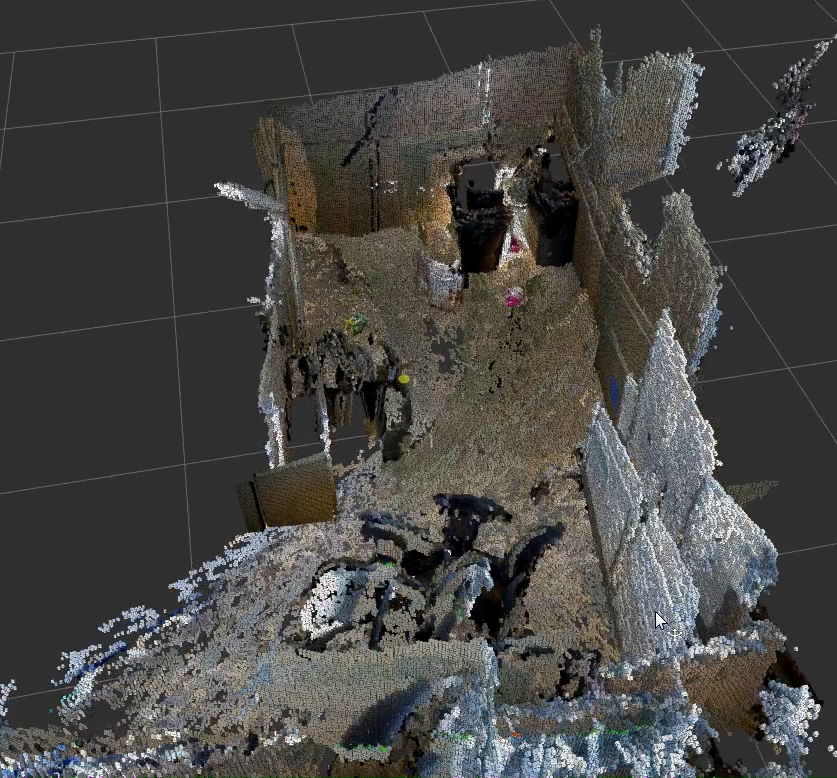
\includegraphics[width=0.4\textwidth]{images/octomap.png}
\caption{Volumetric map of environment built by visual SLAM}
\label{fig:octomap}
\end{center}
\end{figure}

%     ____  _                           _
%    / __ \(_)___________  ____________(_)___  ____
%   / / / / / ___/ ___/ / / / ___/ ___/ / __ \/ __ \
%  / /_/ / (__  ) /__/ /_/ (__  |__  ) / /_/ / / / /
% /_____/_/____/\___/\__,_/____/____/_/\____/_/ /_/
\section{Discussion}
\label{sec:discussion}
%
The experiment demonstrated that our system can autonomously perform complex high-level tasks in an unknown environment. It also revealed several insights on performing high-level tasks with MSRR systems.
\subsection{Challenges}

In order to hold the required sensing and processing resources, the brain module is significantly larger than a regular module. This imposes limitations on possible configurations and locomotion capabilities of the robot. At the same time, the small computer board used in the brain module results in low computation power. Simple configuration designs and efficient algorithms were used to address these issues. To help computation speed further, high-level processing algorithms such as the high-level planner and exploration algorithm were run from external PCs and networked to the robot via WiFi.

Due to power limitations of modules, robot speed is low which results in a long experiment runtime. In addition, the robot is composed of 6 independent robotic components (5 SMORES-EP modules and 1 brain module) which multiplies the chance of a component having a hardware failure. The long runtime combined with multiplied failure points resulted in an increased risk of error occurrences during the experiment. To compensate, repetitive feedback controllers and checks were implemented during task performance. As the robot navigates toward and retrieves objects, it constantly updates its estimate of the object location as new measurements of the object are received. During reconfiguration, docking modules are checked and re-aligned several times during the docking process to ensure they are lined up precisely before connecting to each other. This enables the robot to recover from controller lag and modules dropping velocity commands.

%
\subsection{Reconfiguration}
Our method of reconfiguration has advantages compared to existing methods.  Use of an onboard overhead camera to provide fiducial-based localization for reconfiguration is novel.  This centralized strategy provides localization only near the brain module, so the number of modules that can reconfigure at once is limited by the size of the camera view. In order to scale to large numbers of modules, multiple brain modules would need to be used in parallel.

By exploiting high-fidelity centralized localization and the individual mobility of the SMORES-EP modules, we achieve reconfiguration that is rapid, robust, and cleanly deployable in the context of a high-level task.  In our experiments (Section~\ref{sec:experiments}), we observed that the pre-reconfiguration state required about 20 seconds, each module movement operation required about 45 seconds, and post-reconfiguration required about 10 seconds.
%Each reconfiguration action had a success rate over 90\%.
This compares very favorably with existing methods, in which each reconfiguration action can take on the order of ten minutes \cite{Yim2007},\cite{Murata2006},\cite{Rubenstein2004}.
%\TODO{Verify exact numbers}
%
\subsection{Future Work and Conclusion}
%
The abilities of the system and current MSRR technology could be extended in future work.  Our experiment utilizes a library of two configurations, and our perception system recognizes only three environment types (ledge, tunnel, and free).  To further develop the ability of MSRR systems to adapt to their environment, a larger library of configurations and gait controllers could be designed, along with a more powerful environment characterization algorithm.

The design of a more diverse library of configurations can be greatly aided by improving strength and versatility in module hardware. Real-world applications, such as search-and-rescue, require robots to climb over obstacles and navigate rough terrain. This requires modules with strong locomotion power and the ability to hold large payloads without breaking inter-module connections.

It is important to consider how the presented system could be adapted to work with other modular robot hardware. Our system relies on a 3D sensor for performing RGB-D SLAM, sufficient on-board processing power for perception and control algorithms, and a robust modular hardware system with a versatile self-reconfiguration ability that doesn't rely on external sensors. As long as another MSRR system provides these features and its own hardware-specific and reconfiguration controllers, our system can be integrated into it for performing high-level tasks.

To conclude, this paper presents the first MSRR system that uses perception of an unknown environment to reactively perform complex high-level tasks using intelligent reconfiguration. Components of this system include novel controller synthesis, environment characterization, and self-reconfiguration methods. The demonstration of this novel capability is crucial to the success of modular robots as a technology, and takes a step toward the application of modular robots to tasks in the real world.
%
%\section*{Acknowledgments}
%
%This work was funded by NSF grant numbers CNS-1329620 and CNS-1329692.


       %     ____       ____
       %    / __ \___  / __/__  ________  ____  ________  _____
       %   / /_/ / _ \/ /_/ _ \/ ___/ _ \/ __ \/ ___/ _ \/ ___/
       %  / _, _/  __/ __/  __/ /  /  __/ / / / /__/  __(__  )
       % /_/ |_|\___/_/  \___/_/   \___/_/ /_/\___/\___/____/

%% Use plainnat to work nicely with natbib. 
\bibliographystyle{plainnat}
\bibliography{references}

\end{document}































  


 
